\documentclass[preprint,12pt]{elsarticle}
%\usepackage[numbers,sort&compress]{natbib}
\usepackage{lineno}
\journal{Chemical Engineering Journal}

\usepackage{graphicx}
\usepackage{amsmath}
\usepackage{amssymb}
\usepackage{bm}
\usepackage{color}
\usepackage{tabularx}
\usepackage{overpic}
\usepackage{tikz}
\begin{document}
\begin{frontmatter}
\title{Three-dimensional binary-liquid lattice Boltzmann simulation of microchannels with rectangular
cross sections}
\author[uofa]{A.~Kuzmin\corref{cor1}}
\cortext[cor1]{Corresponding author}
\ead{kuzmin@ualberta.ca}
\author[us]{M.~Januszewski}
\ead{michalj@gmail.com}
\author[schlum]{D.~Eskin}
\ead{deskin@slb.com}
\author[schlum]{F.~Mostowfi}
\ead{fmostowfi@slb.com}
\author[uofa]{J.J.~Derksen}
\ead{jos@ualberta.ca}
\address[uofa]{Chemical and Materials Engineering, University of Alberta\\ 7th Floor, ECERF, 9107
116 St, Edmonton, Alberta, T6G
2V4 Canada}
\address[us]{Insitute of Physics, University of Silesia, 40-007 Katowice, Poland}
\address[schlum]{Schlumberger DBR Technology Center\\ 9450 17 Ave NW, Edmonton, Alberta, T6N 1M9
Canada}
\begin{abstract}
The classical Bretherton problem describes the propagation of gas fingers through liquid media in a
narrow channel with
thin liquid films between bubbles and channel walls. The bubble shape and flow patterns are
complicated functions of the capilary number $Ca$ and Reynolds number $Re$. Recently, we
investigated
an applicability and parameter selection for the two-dimensional Bretherton problem
(flow
between parallel plates) using the free-energy binary liquid lattice Boltzmann method (LBM)
\cite{kuzmin-binary2d}. This paper is the continuation of our previous work with simulations of
three-dimensional channels with rectangular (mostly square) cross sections in the range of the capillary number $0.05\leq
Ca \leq
6.0$.
The flow is driven by a body force, and
periodic boundary conditions are applied in the streamwise direction. The results show that the
binary liquid model is able to correctly capture a number of phenomena occuring in three-dimensional
capillaries, such as the existence of a vortex in front of the bubble and the way bubble radii
depend on the capillary number.  We conclude that lattice Boltzmann free energy binary
liquid model can be used to simulate the Bretherton problem with good accuracy. 
\end{abstract}

\begin{keyword}
Taylor/Bretherton problem \sep Microchannel simulation \sep Multiphase flow \sep Lattice Boltzmann
method
\sep Binary liquid model \sep Flow in microchannels with square cross sections \sep Gravity driven
%% keywords here, in the form: keyword \sep keyword

%% MSC codes here, in the form: \MSC code \sep code
%% or \MSC[2008] code \sep code (2000 is the default)
\end{keyword}

\end{frontmatter}
\linenumbers

\section{Introduction}
The Taylor/Bretherton \cite{bretherton} flow deals with long gas bubbles moving through liquid in
narrow channels. Depending on the channel geometry it was found \cite{gupta-review} that the 
thickness of the liquid film between a bubble and channel walls
is a complicated function of the capillary number $Ca$:
\begin{equation}
\label{capillary:number:definition}
Ca=\frac{U_{\mathrm{bubble}} \mu_{\mathrm{liq}}}{\gamma},
\end{equation}
where $U_{\mathrm{bubble}}$ is the bubble velocity, $\mu_{\mathrm{liq}}$ is the
dynamic liquid viscosity and $\gamma$ is the interfacial tension between gas and liquid. 

For example, the film thickness
is proportional to $Ca^{2/3}$ for small capillary numbers for circular channels
\cite{bretherton,heil-bretherton}. 
Predicting flow patterns and associated mass transfer for Bretheron-type flows
is of significant interest for chemical industry as it is widely used in chemical monolith
microreactors \cite{kreutzer-pressure-drop}. Intensive mass transfer can be achieved because of the
large interfacial area and small diffusion lengths \cite{cerro-bubble-train}. Heat transfer is
also enhanced in comparison with single phase flow \cite{fukugata-levelset}. While it
is possible to calculate the flow analytically for small capillary numbers and nearly zero Reynolds
number \cite{bretherton}, such
results cannot be extrapolated to the wide range of capillary and Reynolds numbers used in the
chemical industry.  Thus, the need of consistent numerical simulations arises.

Flows in two-dimensional geometries (circular tubes, parallel plates) have been studied extensively
in the 
experimental works of \citet{aussillous-deposition}, and \citet{cerro-bubble-train}, and the
numerical works of
\citet{giavedoni-numerical,heil-bretherton}. All abovementioned investigations found that the 
Bretherton
analysis is valid only for small capillary numbers $Ca\leq 0.003$ and deviates from actual
measurements for larger $Ca$.
This is caused by a complex interplay of gravitational,
interfacial, inertial and viscous forces \cite{gupta-review}. Historically, 
\citet{bretherton} neglected inertia effects. \citet{giavedoni-numerical} suggested
that
inertia effects
are negligible for $Ca \leq 0.05$ and have moderate impact for $Ca>0.05$ in the range of Reynolds
number from $0$ to $70$ for two-dimensional flows. Later on, \citet{heil-bretherton}
studied the flow between plates up to $Re=300$. This author noted that while the
influence of inertia on the established film thickness is
insignificant
($7$ percent deviation from the film thickness measured at $Re=0$), the change in Reynolds number
significantly influences  the pressure distrubution and the flow field near the front bubble cap.
\citet{cerro-bubble-train} showed that the mass transfer is strongly affected by flow direction for
small capillary numbers in case of upward and downward flows. Thus, to fully describe the
propagation of the semi-infinite finger in liquid media one needs to take into account the
viscous, gravitational, surface, and inertia forces \cite{gupta-review}.  

In comparison with the two-dimensional Bretherton flows (circular tubes, flow between plates), there
is a vast number of experimental
results available for three-dimensional flows in microchannels with square, triangular and
rectangular cross sections. For instance, \citet{cerro-bubble-train} performed a number of
experiments for a
bubble-train flow in capillaries of square cross sections for horizontal, upward and downward flows.
\citet{shikazono-square} obtained
experimental
results for the film thickness dependence on the
capillary number for ethanol/air and water/air mixtures and for square, circular and triangular
shaped mirochannels. They also presented an experimental correlation for  bubble
radii
based on the capillary number $Ca$ and the Weber number $We=Re\,Ca$, where the Reynolds number is
defined as:
\begin{equation}
Re=\frac{U_{\mathrm{bubble}} H_{\mathrm{eff}}}{\nu_{\mathrm{liq}}},
\end{equation}
where $H_{\mathrm{eff}}$ is the channel height and $\nu_{\mathrm{liq}}$ is the kinematic liquid
viscosity.

The experimental works
\cite{shikazono-square,cerro-bubble-train} supported by numerical simulations \cite{heil-threedim,
wang-non-circular} showed interesting phenomena in three-dimensional geometries. It was found
\cite{heil-threedim,wong-films} that for rectangular capillaries there is a transition from an
asymmetric to an axisymmetric shape for a
certain capillary number.
The non-axisymmetric shape describes the wall normal radius (in Fig.
\ref{fig:lbm:benchmark} the wall normal radius is measured along $x$ or $y$ axes) being 
different from the
diagonal radius and the bubble having a non-circular shape in the channel crossection. In this case,
the bubble shape mimics the shape of a rectangle and looks like a rectangle with rounded corners.
Further we adapt the convention ``axial`` for the radius measured along the $x$ or $y$ axes,
see Fig. \ref{fig:lbm:benchmark} \cite{heil-threedim}. The dependence
of the diagonal and axial radii or a square channel on the capillary number is shown in Fig. 
\ref{fig:heil:three:dim}.
\begin{figure}[htb!]
\begin{overpic}[width=\textwidth]{Figures/capillary_width_heil.eps}
\put(50,45){\includegraphics[width=0.4\textwidth]{Figures/inset.eps}}
\put(20,20){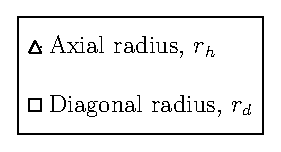
\includegraphics[width=0.3\textwidth]{Figures/legend.eps}}
\end{overpic}
%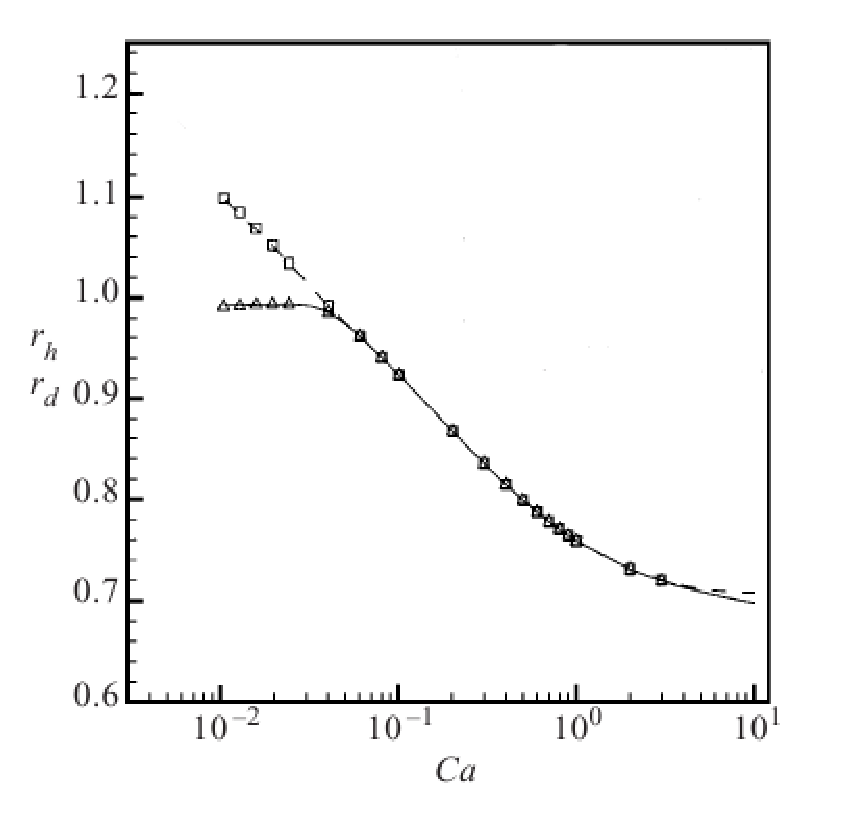
\includegraphics[width=\textwidth]{Figures/capillary_width_heil.eps}
\caption{\citet{heil-threedim} results for the variation of the bubble radii for a range of
capillary numbers for a square channel. One can see the asymmetry between diagonal and axial
diameters for the capillary
numbers $Ca\leq\widehat{Ca}=0.04$. Courtesy of \citet{heil-threedim}. \label{fig:heil:three:dim}}
\end{figure}
The capillary number for square channels at which transition between non-axisymmetric case to
axisymmetric happens is reported in a number of
works ($\widehat{Ca}=0.04$ \cite{cerro-bubble-train},
$\widehat{Ca}=0.1$
\cite{cerro-space,wang-non-circular}, $\widehat{Ca}=0.033$ \cite{heil-threedim}). If the capillary
number is larger
than
the critical capillary number, i.e. $Ca>\widehat{Ca}$, then the bubble becomes axisymmetric with the
radius of the bubble dependent on the capillary number. An example for the bubble radii
dependence on the capillary number is presented in Fig. \ref{fig:heil:three:dim}.

There are also a number of numerical works on three-dimensional flows. For instance, 
\citet{wong-films,wong-pressure} studied
three-dimensional bubbles in
polygonal capillaries and calculated bubble shapes for different
slug and channel cross sections.
\citet{heil-threedim} performed three-dimensional simulations for circular-,
square- and rectangular-shaped capillaries. They indicated a transition of flow regime in a liquid
slug. Vortexes observed at lower capillary numbers disappear as the capillary number goes beyond a
certain threshold,  Fig. \ref{fig:streamlines:pattern}. For a square channel the critical
capillary number is $Ca=0.691$.  \citet{heil-threedim} also found an empirical
correlation which
makes it possible to collapse results of radii dependency on the capillary number
simulations of rectangular channels with different aspect ratios on a single curve.
It was also found that for microchannels with a certain aspect ratio $\alpha=\frac{a}{b}\geq
2.04$, the interface does not become
circular for any capillary number. \citet{wang-non-circular} performed numerical
simulations using the Volume of Fluid (VOF) technique for
capillaries with non-circular (square, triangular) cross sections. They also investigated the
relative slug to bubble velocity for
a range of capillary numbers. 

As was mentioned by \citet{gupta-review}, the most common techniques to simulate the Bretherton
phenomena are the VOF method \cite{wang-non-circular}, the level-set method
\cite{fukugata-levelset} and the finite element methods \cite{kreutzer-taylor,heil-threedim}. It was
also indicated \cite{gupta-review} that the new techniques, which are still in the development
stage,
are the lattice Boltzmann method and phase field methods \cite{anderson-diffuse,gurtin-binary}.
The finite element method solves the Bretherton flow as a free-surface problem with a sharp
interface but without gas.  The lattice Boltzmann method is a continuous
interface method, and therefore provides more flexibility in simulations involving coalescence
and/or
droplet breakup, and thus arises as a promising alternative for simulation of gas finger propagation. 

In our previous work \cite{kuzmin-binary2d}, we already analyzed the Bretherton flow between
parallel
plates.
It was shown that the free-energy binary liquid model, which is a phase field method, simulates the
Bretherton/Taylor phenomenon with reasonable accuracy. The goal of this work is to examine 
if similar conclusions can be drawn for three-dimensional flows in microchannels with square cross
sections,
simulated using the free-energy binary liquid lattice Boltzmann
method. 
%As it was indicated by \citet{gupta-review} the flow in microchannels is a complex
%interplay of viscous, gravitational, inertial and surface forces. For the sake of comparison, we
%specifically design the numerical benchmark to avoid the influence of gravitational and inertial
%forces.


The lattice Boltzmann method has emerged as a successful method to simulate
a wide variety of phenomena including hydrodynamics \cite{yu}, thermal flows
\cite{karlin-minimalmodels}, microflows \cite{ansumali-small-knudsen},
ferrofluids \cite{kuzmin-aniso}, and multiphase flows
\cite{swift,Shan-chen:extended}. The method is a particle method which allows one to simulate physical
phenomena on the microscopic level. For instance, the introduction of the force or potential on the
microscopic level allows to restore multiphase macroscopic equations \cite{swift,
Shan-chen:extended}.

The binary liquid free-energy LB model due to \citet{swift} that we used
simulates two liquids with the assumption of uniform overall
density. %As it was indicated by \citet{gupta-review} a flow in microchannels is a complex
%interplay of viscous, gravitational, inertial and surface forces. 
The classical Bretherton
problem is stated for gas and liquid, which are of
significantly
different density and viscosity. However, the numerical results of
\citet{giavedoni-numerical} and \citet{heil-bretherton} show
negligible Reynolds number effects on the film thickness for a relatively wide range of Reynolds
numbers, $Re<70$. The parameters in our simulations were carefully chosen to
avoid  inertia
effects, see Section \ref{sec:numerical:benchmark}. The maximum attained
Reynolds number $Re<10$. Thus, inertia effects can be neglected. Therefore, a major governing
factor for microchannel flows is not the density ratio, but
the
viscosity ratio. As a result, the uniform density binary liquid model is suitable for this kind of
simulations.  
% THIS HAS ALREADY BEEN STATED BEFORE
% The goal of this work is to do a feasibility study of the LBM
% binary-liquid model to simulate and correctly predict flow patterns for the Bretherton/Taylor
% problem. 

% TODO: This sentence should probably be moved to a summary/conclusions section?
%The work results are in good agreement with other simulations
%\cite{heil-threedim,wang-non-circular}.

One should acknowledge the works of \citet{pagonabarraga-fingers} on menisci
in thin films for fingering phenomena. \citet{sehgal-microchannel} performed lattice Boltzmann
simulations of two-dimensional channel flows for relatively large capillary numbers, and
found discrepancies with the classical Bretherton theory, which
is limited to the low capillary number regime \cite{giavedoni-numerical}. They used the Shan-Chen model,
 which is sometimes said to contain a thermodynamically
inconsistent interface \cite{nourgaliev-breakup}. 

The paper is organized as follows.  First, we explain the simulation benchmark construction
mainly based on our previous work \cite{kuzmin-binary2d}. Then, the binary liquid lattice
Boltzmann model is outlined. The simulation results for the three-dimensional case are presented in
the results section. That covers the film thickness dependency on the capillary number, the bubble
to slug relative velocity and vortex profiles for square microchannels. We also briefly cover flow
simulations for rectangular channels. The paper
is concluded with a summary of the main findings.
%The critical capillary numbers for changing velocity pattern depending on the eccentricity
%parameter $\alpha$ are presented in Table \ref{table:recirculation:data}.
%\begin{table}
%\begin{tabular}{c|c}
%$\alpha$& $Ca_{T}$\\
%\hline
%1& 0.691\\
%1.1 & 0.688\\
%1.3 & 0.666\\
%1.5 & 0.631\\
%\end{tabular}
%\caption{The results for the recirculation region.\label{table:recirculation:data}}
%\end{table}

\section{Numerical benchmark approach}
\label{sec:numerical:benchmark}
The main discussion here is based on the two-dimensional benchmark approach
\cite{kuzmin-binary2d}. It was indicated that the benchmark layout should have certain
dimensions to conduct simulations. The classical Bretherton benchmark layout is represented in
Fig.~\ref{fig:classical:benchmark}. It describes the gas finger propagation through the liquid
medium.
The film thickness in this case is measured at the inlet. In the lattice Boltzmann framework, such a
formulation has certain challenges \cite{kuzmin-binary2d}. Some of them are attributed to the
dynamic coupling of the inlet and outlet conditions \cite{giavedoni-numerical}. Instead, we
proposed the numerical benchmark indicated in Fig.~\ref{fig:lbm:benchmark}. The dimensions of the
channel are chosen as $H_{\mathrm{eff}}\times H_{\mathrm{eff}} \times 15 H_{\mathrm{eff}}$. The
initial bubble length is taken as $5 H_{\mathrm{eff}}$. \citet{giavedoni-numerical} showed that
the film in the two-dimensional geometry stabilizes at distances of $2.6-4.0$ diameters
from the front tip depending on the Reynolds number. \citet{heil-threedim} measured the bubble radii
at the distance of $5.5 H_{\mathrm{eff}}$ and indicated it to be sufficient for $Ca\leq 10$. In
this work, the following relation holds for all conducted simulations: $0.05 \geq Ca \leq 6$.
Thus, the
film thickness is chosen to be measured in the
middle of the bubble, which is located at least at a distance of $2.5-3$ channel heights from the 
bubble tip.%at the distances one channel height from the rear tip upto one channel

For simplicity, periodic boundary conditions are applied. Therefore  a bubble
train is simulated
instead of a single bubble.  The mutual influence of neighbouring bubbles is minimized
by using a long
channel ($15 H_{\mathrm{eff}}$). Periodic boundary conditions imply as well that the fluid is driven
by a
body force in the framework of the LBM and not with a pressure difference. Therefore, we can not
address simulations with upward and downward flows \cite{cerro-bubble-train} which would require a
simultaneous imposement of pressure boundary conditions and the body force. 
%The pressure boundary
%conditions for the binary liquid model is a challenge. Thus, we consider a flow in the
%horizontal direction only and the upward/downward flows with pressure difference imposed are not
%simulated. 
\begin{figure}[htb!]
\includegraphics*[bb=153 610 410 717,width=\textwidth]{Figures/benchmark_classical.eps} 
\caption{The classical benchmark layout describes a semiinfinite gas bubble
propagation through the liquid media. The inlet pressure is specified $P_{in}$, the outlet is the
free outflow. The bubble propagates with constant velocity $U_{\mathrm{bubble}}$. 
\label{fig:classical:benchmark}}
\end{figure}
\begin{figure}[htb!]
\includegraphics*[bb=152 470 415 713,width=\textwidth]{Figures/benchmark_lbm.eps}
\caption{The lattice Boltzmann benchmark layout as used in present calculations. The dimensions of
the domain are chosen as $H_{\mathrm{eff}}\times H_{\mathrm{eff}}\times 15 H_{\mathrm{eff}}$. The
length of the bubble was chosen as $5 H_{\mathrm{eff}}$ for the film thickness to stabilize.
Periodic boundary conditions are applied in the streamwise direction. The flow is driven by a body
force. \label{fig:lbm:benchmark}}
\end{figure}

It was indicated \cite{kuzmin-binary2d} that the film thickness for two-dimensional simulations should be at least twice as large
as the interface thickness. The interface thickness occupies $3-5$ nodes due to the continuous
interface formulation of the binary liquid model. Therefore, the
film should be
resolved as at least $6-10$ nodes. 

\citet{heil-threedim} and Fig. \ref{fig:heil:three:dim} specify that the diagonal bubble radius is
different from the
axial bubble radius for $Ca\leq \widehat{Ca}\approx 0.03$. The radii are approximately the same for
larger values
of
$Ca$ with a value $R_{diag}=R_{axis}=0.49 H_{\mathrm{eff}}$. Therefore, taking the minimal
requirement for the film thickness to be
resolved, i.e. $6$ lattice nodes, one would obtain a grid size of $600\times 600 \times 9000 $ to
properly resolve the binary liquid flow. This size implies that relatively
large
computational resources are required to perform the simulations.

One can argue that a non-uniform grid could be used. However, the film thickness is a
function of the curvatures of the front bubble tip \cite{bretherton} and the grid would need to
be refined just at the interface between gas and liquid. This is complicated to achieve for
dynamic systems where a bubble moves in the streamwise direction.
To reduce the computational overhead, we decided to take a simpler approach and exploit the
inherent symmetry of the problem by simulating only a quarter of the channel (see
\ref{append:sym} for details).

% TODO: This paragraph should be revisited, somehow it reads a little weirdly..
It should be noted that the binary liquid model we used has a uniform density. This issue was
partially addressed in the introduction:  to describe the Bretherton problem one needs to take into
account gravitational, viscous, inertial, and surface tension forces. Among all the works, there
is no full 
agreement between results even in the limit of Reynolds number zero. Moreover,
as was indicated
by \citet{kreutzer-taylor} and by \citet{cerro-bubble-train} the pressure distribution, streamlines
and bubble shape are strongly affected by the length of the liquid slug and the length of the
bubble. In the current simulations we minimize the effects of bubbles train and inertia. Inertia
effect are minimized as the largest Reynolds number is not bigger than $10$. The mutual
effects of bubbles motion on each other is minimized by choosing lengths of a bubble and a
channel large enough in comparision with the channel height. However, more thorough studies are
needed in order to understand
precisely the abovementioned effects.

%However, 
%\citet{shikazono-square} indicated that for square-shaped capillaries the bubble radii have the
%following dependency on the capillary number $Ca$ and the Weber number $We$:
%\begin{equation}
%\label{radii:experimental}
%\begin{aligned}
%&R_{diag}=1.171-\frac{2.43 Ca^{2/3}}{1+7.28 Ca^{2/3}-0.255 We^{0.215}}\\
%&R_{axis}=
%\begin{cases}
%1, &R_{diag}>1\\
%R_{diag}, &R_{diag}\leq 1.
%\end{cases}
%\end{aligned}
%\end{equation}
%Equation (\ref{radii:experimental}) shows that a change in the Reynolds number $0\leq Re \leq 100$
%implies the change of the radii from $R_{diag}=R_{axis}=0.96$ to $0.93$ for $Ca=0.1$ and from
%$R_{diag}=R_{axis}=0.88$ to $0.85$ for $Ca=1.0$. The error of $3$ percent of the channel height is
%acceptable for current simulations where the Reynolds number is less than $10$.

% AGAIN, THIS IS REPEATS WHAT HAS ALREADY BEEN SAID
%Thus, having limitations of the computational memory and performance requirements the focus of the
%present work is a feasibility study of the binary liquid lattice Boltzmann method for the
%microchannel simulations with square crossections conducted in the moderate capillary number range
%$0.1 \leq Ca \leq 1.0$. We base our work on comparison with the already available studies. 

%The next section briefly explains the binary liquid lattice Boltzmann model.
%The steady-state approach, the dependency of the radii on the moderate capillary number values
%$0.05\leq Ca \leq 6.0$, the velocity pattern, and the relative to the liquid slug bubble velocity 
%are discussed in Section
%\ref{sec:results}. 

\section{Binary liquid lattice Boltzmann model}
The lattice Boltzmann equation (LBE) operates on a rectangular grid representing the
physical domain. It utilizes
probability distribution functions (also known as particle populations)
containing information about
macroscopic variables, such as fluid density and momentum. LBE consists of
two parts: a local collision step, and a propagation step which transports
information from one node to another in certain
directions specified by a discrete velocity set.
The LBE is typically implemented as follows \cite{ginzburg-boundary-main}:
\begin{equation}
\label{standard:implementation}
\begin{aligned}
&f_i^{*}(\bm{x},t)=\omega f_i^{eq}(\bm{x},t)-(1-\omega) f_i(\bm{x},t) +
F_i,&&\text{collision step}\\
&f_i(\bm{x}+\bm{c_i},t+1)=f_i^{*}(\bm{x},t),&&\text{propagation step}\\
&g_i^{*}(\bm{x},t)=\omega_{\phi} g_i^{eq}(\bm{x},t)-(1-\omega_{\phi})
g_i(\bm{x},t),&&\text{collision step}\\
&g_i(\bm{x}+\bm{c_i},t+1)=g_i^{*}(\bm{x},t),&&\text{propagation step},
\end{aligned}
\end{equation}
where $\{f,g\}_i$ are the probability distribution functions in the direction $\bm{c_i}$, $\omega$
is the
relaxation parameter, $\omega_{\phi}$ is the phase relaxation parameter, and $F_i$ is the external
force population responsible for force inclusion to the Navier-Stokes equation.

The binary fluid LB model is
based on a free-energy functional \cite{swift,landau}, and operates with two
sets of populations: one ($f_i$) to track the pressure and the velocity fields, and another ($g_i$) to represent the
phase field $\phi$ indicating gas or liquid.
The equilibrium populations \cite{pooley-contact} are defined as:
\begin{equation}
\label{set:equilibrium:binary}
\begin{aligned}
&f_i^{eq}&&=w_i 
\biggl(3
p_0 - k \phi \Delta \phi
+\frac{u_{\alpha}c_{i\alpha}}{c_s^2}+\frac{Q_{i\alpha\beta}u_{\alpha } u_ {
\beta}}{2 c_s^4}\biggr)\\
&&&+k w_i^{\alpha\beta} \partial_{\alpha} \phi\partial_{\beta} \phi, 1\leq i \leq Q-1\\
&f_0^{eq}&&=\rho-\sum_{i\neq0}{f_i^{eq}}\\
&g_i^{eq}&&=w_i\left(\Gamma \mu + \frac{\phi c_{i\alpha} u_{i\alpha}}{c_s^2}+\phi
\frac{Q_{i\alpha\beta}u_{\alpha}u_{\beta}}{2 c_s^4}\right), 1 \leq i \leq Q-1\\
&g_0^{eq}&&=\phi-\sum_{i\neq0}{g_i^{eq}}\quad,
\end{aligned}
\end{equation}
where $\Gamma$ is the mobility parameter; the chemical potential
$\mu=-A\phi+A\phi^3-k\Delta\phi$; $k$ is a parameter related to the surface
tension; $A$ is a parameter of the free-energy model; $Q$ is the number of directions ($19$
for the $D3Q19$ model); the tensor
$Q_{i\alpha\beta}=c_{i\alpha} c_{i\beta} - c_s^2 \delta_{\alpha\beta}$ with
the sound speed parameter $c_s^2=1/3$. The bulk pressure
is expressed as $p_0=c_s^2 \rho +A (-0.5 \phi^2+0.75 \phi^4)$. The discrete velocity set is defined as:
\begin{equation} 
\begin{aligned}
&c_{ix}=\{0,1,-1,0, 0,0, 0,1,-1, 1,-1,0, 0, 0, 0,1,-1, 1,-1\}\\
&c_{iy}=\{0,0, 0,1,-1,0, 0,1, 1,-1,-1,1,-1, 1,-1,0, 0, 0, 0\}\\
&c_{iz}=\{0,0, 0,0, 0,1,-1,0, 0, 0, 0,1, 1,-1,-1,1, 1,-1,-1\}.
\end{aligned}
\end{equation}
The weights are $w_0=0$, $w_{1-6}=\frac{1}{6}$ and $w_{7-18}=\frac{1}{12}$. The weights
related to the inclusion of the surface tension are:
\begin{equation}
\begin{aligned}
&w^{xx}_{1-2}=w^{yy}_{3-4}=w^{zz}_{5-6}=\frac{5}{12}\\
&w^{xx}_{3-6}=w^{yy}_{1-2,5-6}=w^{zz}_{1-4}=-\frac{1}{3}\\
&w^{xx}_{7-10,15-18}=w^{yy}_{7-14}=w^{zz}_{11-18}=-\frac{1}{24}\\
&w^{xx}_{11-15,}=w^{yy}_{15-18}=w^{zz}_{7-10}=\frac{1}{12}\\
&w^{xy}_{7,10}=-w^{xy}_{8,9}=w^{yz}_{11,14}=-w^{yz}_{12,13}=w^{zx}_{15,18}=-w^{zx}_{16,17}=\frac{1}{
4}.
\end{aligned}
\end{equation}

The set of equations (\ref{set:equilibrium:binary}) restores the macroscopic
fluid equations as:
\begin{equation}
\label{full:navier:stokes}
\begin{aligned}
&\partial_t \rho+ \partial_{\alpha} \rho u_{\alpha}=0\\
&\rho\left(\partial_t+u_{\beta}\partial_{\beta}\right) u_{\alpha}=F_{\alpha}
-\partial_{\beta}P_{\alpha \beta} +
\nu\partial_{\beta}\left(\rho\partial_{\alpha}u_{\beta}+\rho\partial_{\beta} u_{\alpha}\right)\\
&\partial_t \phi + \partial_{\alpha} \phi u_{\alpha}=M \partial^2_{\beta\beta} \mu,
\end{aligned}
\end{equation}
where $\nu=c_s^2 (\tau-1/2)$ is the kinematic viscosity,
$M=\Gamma(\tau_{\phi}-1/2)$ is the mobility parameter, and $\tau=\frac{1}{\omega}$ and
$\tau_{\phi}=\frac{1}{\omega_{\phi}}$
are the relaxation parameters of density and phase fields. The first equation of system
(\ref{standard:implementation}) simulates the continuity equation and the Navier-Stokes equation.
The lattice Boltzmann equation for the second set $g_i$ simulates the phase propagation with the
supplied velocity from the Navier-Stokes equation.

The system allows the separation of the liquid
phase with $\phi=1$ and a so-called gas phase with $\phi=-1$. The
relaxation time is taken to be linearly dependent on the relaxation
times $\tau_{\mathrm{gas}}$ and $\tau_{\mathrm{liq}}$:
$\tau=\tau_{\mathrm{gas}}+\frac{\phi+1}{2}(\tau_{\mathrm{liq}}-\tau_{\mathrm{gas}})$. This
makes it possible to smoothly change viscosity from the gas viscosity
$\nu_{\mathrm{gas}}=\frac{1}{3}\Bigl(\tau_{\mathrm{gas}}-\frac{1}{2}\Bigr)$ to the liquid viscosity
$\nu_{\mathrm{liq}}=\frac{1}{3}\Bigl(\tau_{\mathrm{liq}}-\frac{1}{2}\Bigr)$ in a region where a
phase gradient exists. The surface tension in the framework of the binary liquid model is $\sqrt{\frac{8 k
A}{9}}$.

\section{Results}
\label{sec:results}
This section describes numerical simulations. We refer to \ref{append:scaling} for
initialization and scaling procedures. The simulations were conducted on the following 
fluid domain grids $100 \times 100 \times 1500$, $160 \times 160 \times 1500$,
$160 \times 160 \times 2400$ and $200 \times 200 \times 3000$. Body forces were varied as
$\frac{\mathrm{d}P}{\mathrm{d}z}=10^{-6}-10^{-4}$ lattice units. The binary-liquid model parameters
were kept in
the stable region $k=A=0.004,0.04$. The relaxation rates were taken as $\tau_{\mathrm{liq}}=2.5$
and $\tau_{\mathrm{gas}}=0.7$ giving a gas-over-liquid viscosity ratio of $10$. The relaxation
parameter for the phase field was $\tau_{\phi}=1.0$.

First, we examine when the steady-state is
reached. Then, the critical capillary number is identified where the transition from the
non-symmetrical to axisymmetrical bubble shape occurs. The dependency of the radii on the capillary
number is presented for the range of moderate capillary numbers $0.05 \leq Ca \leq 6.0$. Results are
concluded with studies of the velocity pattern.

\subsection{Steady-state approach}
\label{sec:steady:state}
We performed different simulations to understand the number of time steps required for the
system to
settle down to a steady state. The grid  was $52 \times 52 \times 750$ which represents
a quarter of the channel with the initial film thickness of $6.5$ lattice units together
with the body force $\frac{\mathrm{d}P}{\mathrm{d}x}=1.6
\cdot 10^{-6}$. The simulation was performed for $250000$ iterations with the step of
$10000$ iterations. The results for time iterations $140000-250000$ are summarised in Table
\ref{table:steady:state}. While the
capillary number variation is around $5$ percent, the radii variation is $0.1$ percent. Note, that
the interface velocity is defined as the bubble tip velocity in the microchannel center. Multiphase
lattice Boltzmann models is known to have spurious currents near the interface
\cite{pooley-spurious,shan-spurious}. Therefore, the bubble interface velocity is influenced by
spurious currents and capillary numbers show larger variation than radii. 
\begin{table}
\begin{tabularx}{\textwidth}{|X|X|X|X|}
\hline
$N_{iter}$&$Ca$&$R_{axis}$&$R_{diag}$\\
\hline
$140000$&$0.1879$&$0.8657$&$0.8708$\\
$150000$&$0.1879$&$0.8652$&$0.8704$\\
$160000$&$0.1878$&$0.8650$&$0.8702$\\
$170000$&$0.1880$&$0.8648$&$0.8701$\\
$180000$&$0.1882$&$0.8647$&$0.8700$\\
$190000$&$0.1885$&$0.8646$&$0.8699$\\
$200000$&$0.1893$&$0.8645$&$0.8698$\\
$210000$&$0.1963$&$0.8645$&$0.8697$\\
$220000$&$0.1925$&$0.8644$&$0.8697$\\
$230000$&$0.1936$&$0.8644$&$0.8697$\\
$240000$&$0.1961$&$0.8645$&$0.8697$\\
$250000$&$0.1932$&$0.8645$&$0.8698$\\
\hline
\end{tabularx}
\caption{Results for the steady-state case. One
can see that $200000$ steps are enough to shape
the bubble and approach the steady state. The small noise in the capillary number is connected to
the identification of the interface and spurious currents in the system. The spurious currents
influence the bubble velocity identification which is taken at the front bubble tip. The binary
liquid model is the continuous interface model. Thus one needs to interpolate phase function data to
obtain the location of the bubble interface $\phi=0$ and its velocity. Thus, there is a larger
deviation for capillary numbers. All other parameters are relaxed to the
steady-state.\label{table:steady:state}}
\end{table}

To further examine the steady-state, the velocity in the streamwise direction is plotted. The values
of the velocity are taken on the contour where $\phi=0$. This corresponds
 to the bubble interface. That allows to check whether the bubble is propagating as a whole rigid
body or it's shrinking or elongating. This is one of the characteristics of the steady-state.  One
can see in Fig. \ref{fig:velocity:contour} the contour plot and the
corressponing streamwise velocity
component. The crossection is a plane $x=0$, where $x$ points
towards the reader, $z$ is the streamwise direction. As fluxes inside the bubble have
clockwise and counterclockwise directions, see Section \ref{sec:velocity}, one needs to thoroughly
examine only the points corresponding to the front and the rear bubble caps. If they are equal, then
it is exactly the velocity with which the bubble propagates in the microchannel as a rigid body.
For a physical analogy, one can imagine the rotating ball propagating in the streamwise direction.
The front and rear ball points have the same streamwise velocity. 
\begin{figure}[ht]
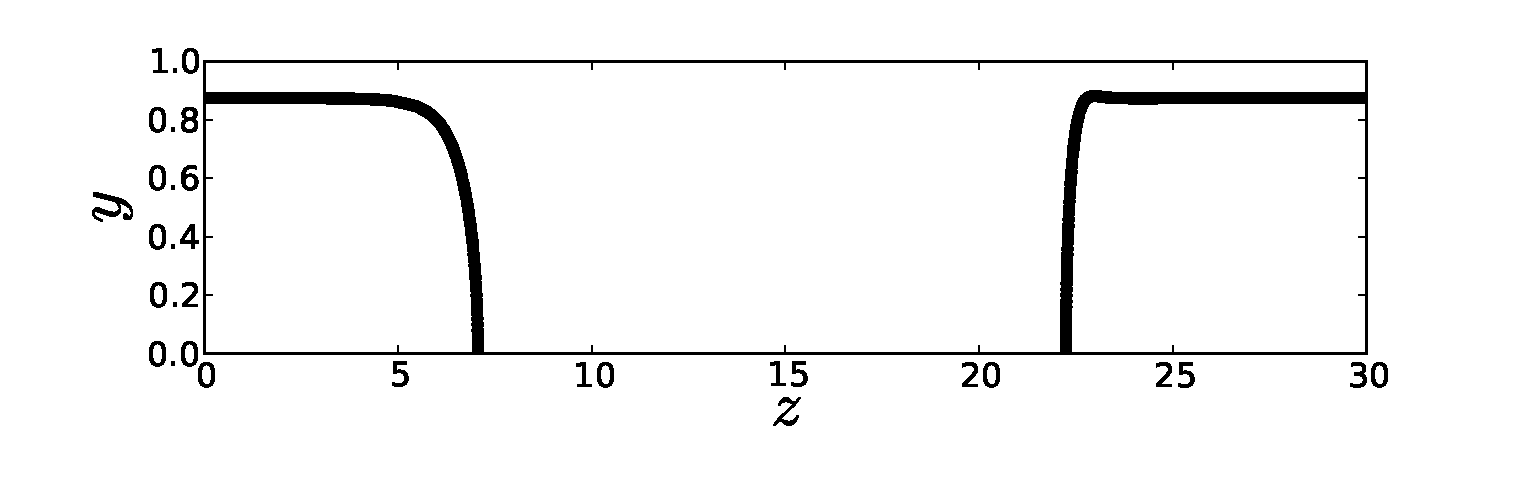
\includegraphics[width=\textwidth]{Figures/velocity_interface_contour.eps}\\
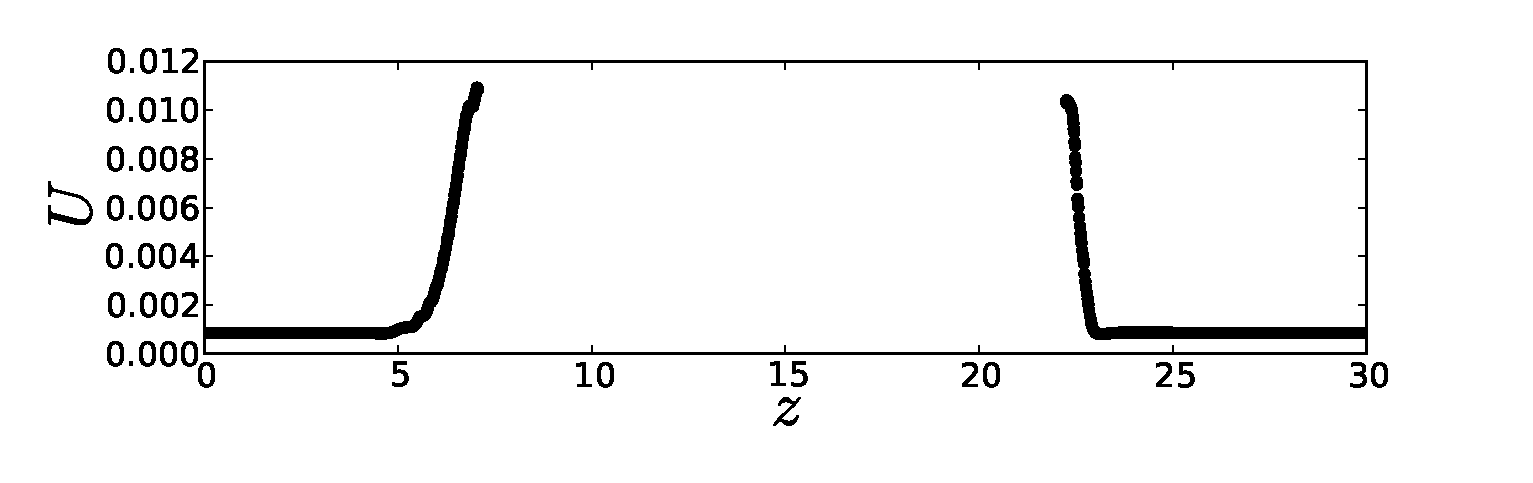
\includegraphics[width=\textwidth]{Figures/velocity_interface_values.eps}\\
\caption{The bubble shape and the corresponding streamwise velocities taken on the bubble
interface after $240000$ iterations. Directions $y$ and $z$ are scaled to the half of the channel
$H_{\mathrm{eff}}/2$. One can see that the bubble front and rear caps are propagating with nearly
the
same velocity, that is the actual bubble velocity. For more details on velocity patterns
see Section \ref{sec:velocity}. \label{fig:velocity:contour}}
\end{figure}


\subsection{Radii transition}
Due to computational power restrictions we can only access the
region of $Ca\geq 0.05$. In this region the proper resolution of the film thickness
is achievable.  To identify the critical capillary number $\widehat{Ca}$ a number of
simulations
were conducted, see Table \ref{table:transition:results}. In comparison with the results of the
\citet{heil-threedim}
($\widehat{Ca}=0.04$) our
results are closer to the VOF continuous interface method simulation by
\citet{wang-non-circular} ($\widehat{Ca}=0.1$). Due to linear approximation we consider a bubble to have a circular cross section if $R_{axis}$ and $R_{diag}$ differ by less than $1\%$. The transition for current simulations
happens for $Ca\approx 0.09$ calculated as linear interpolation between data presented in Table
\ref{table:transition:results}. 
%Our data also fall within $5$ percent radii
%variation on the
%capilllary number of experimental dependency of
%\citet{shikazono-square}.   
One can see
two examples of non-axisymmetric and axisymmetric bubble shapes for $Ca=0.053$ and $Ca=1.13$, see
Fig.
\ref{fig:crosssections:sym}.  
\begin{table}
\begin{tabularx}{\textwidth}{|X|X|X|X|}%X|X|}
\hline
$Ca$&$R_{axis}$&$R_{diag}$&$Re$\\ %&$R_{axis,Wang}$&$R_{diag,Wang}$\\
\hline
$0.053$&$0.95$&$1.01$&$0.907$\\%&$0.99$&$0.99$\\
$0.078$&$0.93$&$0.95$&$1.062$\\%&$0.96$&$0.96$\\
$0.102$&$0.91$&$0.91$&$1.392$\\
$0.132$&$0.89$&$0.89$&$1.80$\\%&$0.93$&$0.93$\\
\hline
\end{tabularx}
\caption{Simulation results in terms of $R_{axis}$ and $R_{diag}$ for the transition region between
non-axisymmetric and axisymmetric cases. The transition occurs at $\widehat{Ca}=0.09$, which is a
linear interpolation between data with radii not equal and equal to each other. The grid for
simulations was chosen as $50\times50\times1500$ for a quarter of a channel. That means that the
corresponding interpolation error of determining radii is a half of the reverse grid number,
$\frac{1}{2 N_x}=0.01$. Thus, if radii values are within $1$ percent we consider them equal to
each other. We also included a corresponding Reynolds number to show that inertia effects can be
neglected.
\label{table:transition:results}}
\end{table}
\begin{figure}[ht]
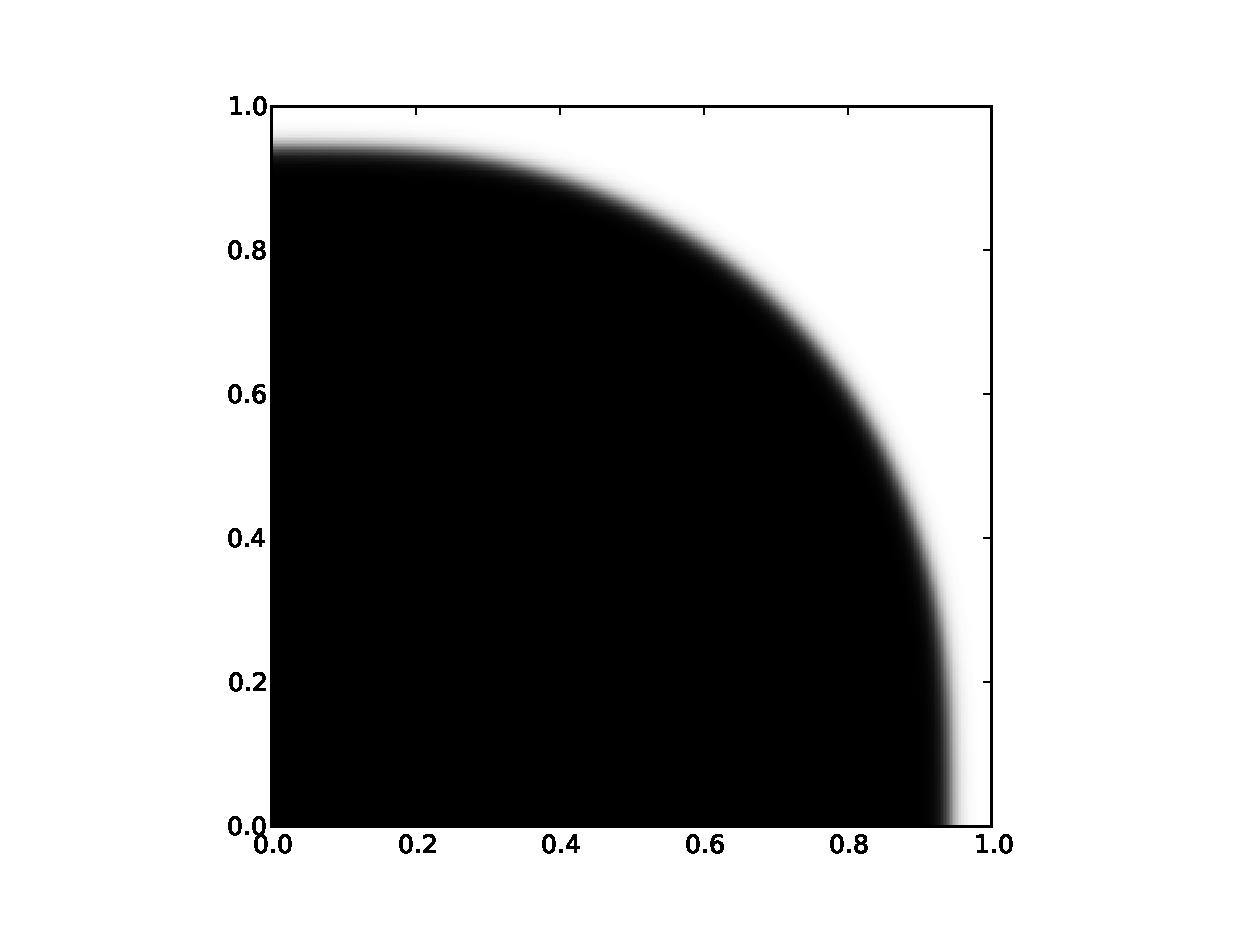
\includegraphics[width=0.5\textwidth]{Figures/phase_crossection_ca5.eps}
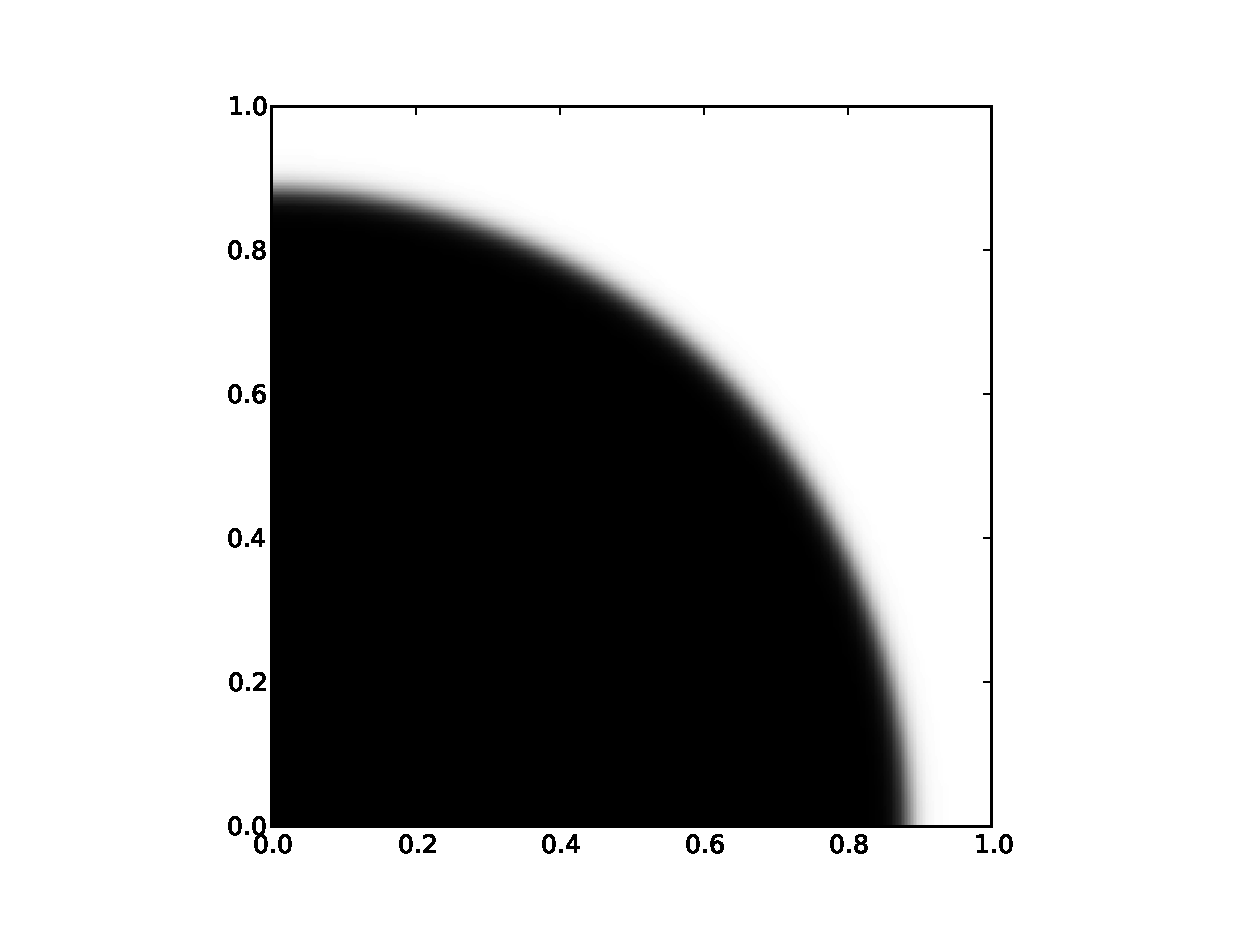
\includegraphics[width=0.5\textwidth]{Figures/phase_crossection_ca13.eps}\\
\caption{Crosssections of the phase field in the middle of the bubble for $Ca=0.053$
(left) and $Ca=1.13$ (right). Crosssections are rescaled on the half channel height. Other
parameters are indicated in Table \ref{table:transition:results}. One can see that the left picture
is non-axisymmetric in contrast
with the right one, i.e. $R_{diag}\neq R_{axis}$. The transition happens at
$\widehat{Ca}=0.09$.\label{fig:crosssections:sym}}
\end{figure}


\subsection{Velocity pattern}
\label{sec:velocity}
The liquid velocity pattern is known to change its behavior depending on the capillary number. For
relatively low capillary numbers $Ca<0.6$, in a reference frame moving with the bubble a vortex 
is observed \cite{heil-threedim}. For larger capillary numbers it is indicated that there is no
vortex in front of the bubble. The transition capillary number specified by
\citet{heil-threedim} for a square channel as $Ca=0.691$. However, the
distribution of vorticity strongly depends on the Reynolds number \cite{heil-bretherton}, as well as
on
the
pressure distribution. In the case of the bubble train it is indicated by \citet{kreutzer-taylor}
that the pressure is significantly influenced by bubble frequency and slug distance. The present
simulations are conducted for bubble trains and certain differences in terms of changing streamline
patterns are expected. We examined velocity patterns to identify the moment of the streamlines
pattern change. We chose two
representative capillary numbers as $Ca=0.47$ and $Ca=0.63$. 
One can
see in Fig. \ref{fig:streamlines:pattern} a clear transition between associated patterns. Among all
different simulation runs with different grids and initial conditions, the
transition occurs at $Ca=0.6-0.7$, see Fig. \ref{fig:streamlines:pattern}. The
transition is identified between regimes where there exists and does not exist a vortex in the
slug. Either all streamwise slug velocities have the same sign (no vortex), or have different signs
(vortex). It is indicated by \citet{heil-bretherton,kreutzer-reactors} that the bubble train flow
depends on the slugs and bubbles lengths. Thus, we expect the difference of bubble train simulations
and simulations of a semi-infinite air finger propagation \cite{heil-threedim}. The transition also
depends on the identification of the bubble velocity
which is influenced by spurious currents and interpolation errors.
\begin{figure}[ht]
\includegraphics[angle=90,width=\textwidth]{Figures/stream_ca47.eps}\\
\includegraphics[angle=90,width=\textwidth]{Figures/stream_ca63.eps}\\
\caption{Velocity vector maps for $Ca=0.47$ and $Ca=0.63$. One can see that there are no vortexes
created
in front of the bubble for $Ca=0.63$. For presented simulations the transition happens between
$Ca=0.47$ and $Ca=0.63$, which
is a different value from $Ca=0.69$ \cite{heil-threedim}. However, we performed a number of
different types of simulations (different force, width initialization). The critical transition
capillary number $\widehat{Ca}$ is not well fixed and varies from $\widehat{Ca}=0.6-0.7$.  
\label{fig:streamlines:pattern}}
\end{figure}

\subsection{Variation over bubble length}
The work of \citet{wang-non-circular} shows the variation of the bubble
radii along the
bubble. The bubble shape in terms of axial and diagonal radii is reconstructed for a number of
capillary numbers, Fig. \ref{fig:bubble:variation:capillaries}. One can see that for smaller
capillary numbers the diagonal radius exhibits a small jump near the rear bubble cap. That agrees
with results of \citet{wang-non-circular}. However, our simulations show smoother behavior of
the jump.  
\begin{figure}[ht]
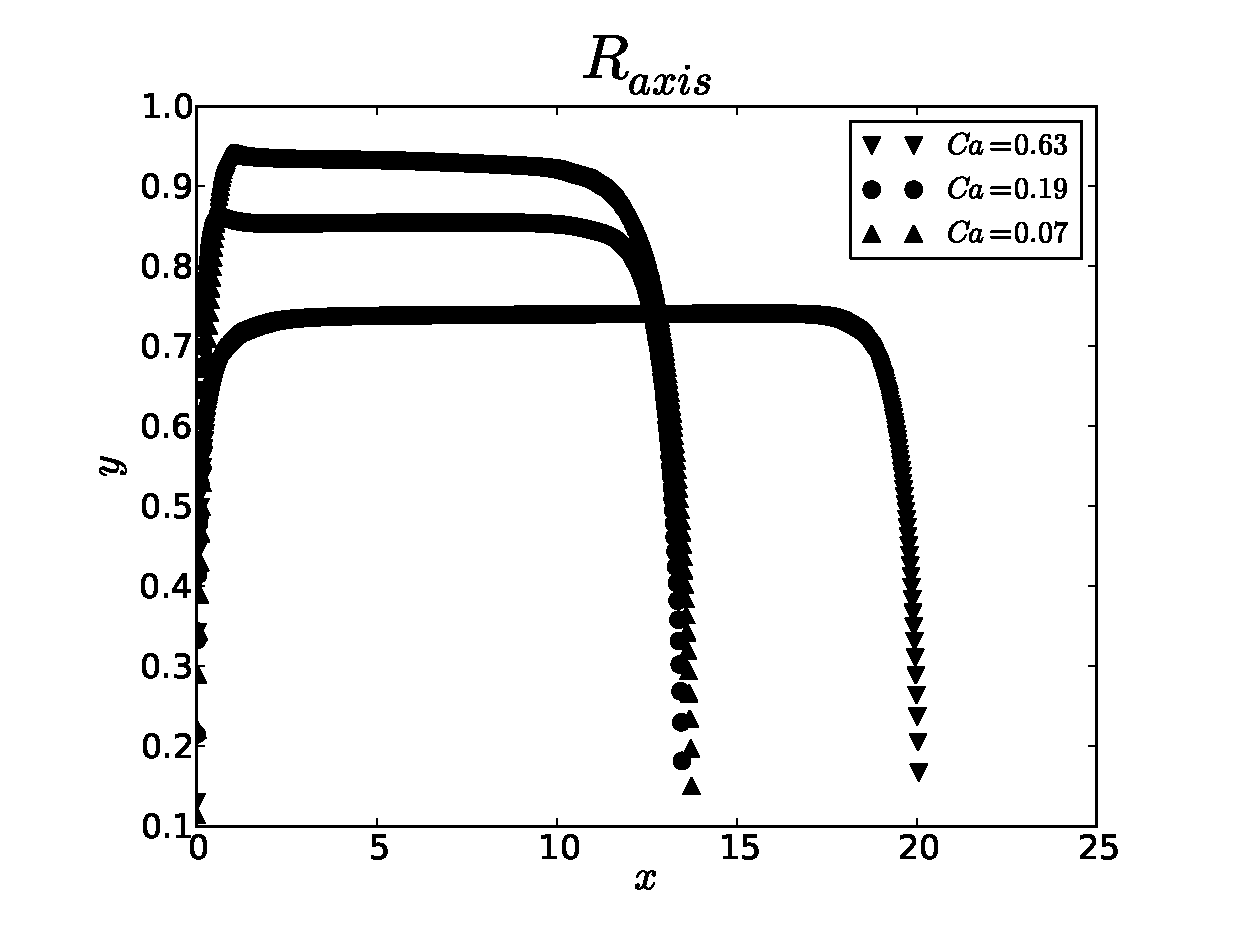
\includegraphics[width=0.8\textwidth]{Figures/bubble_rad_axis.eps}\\
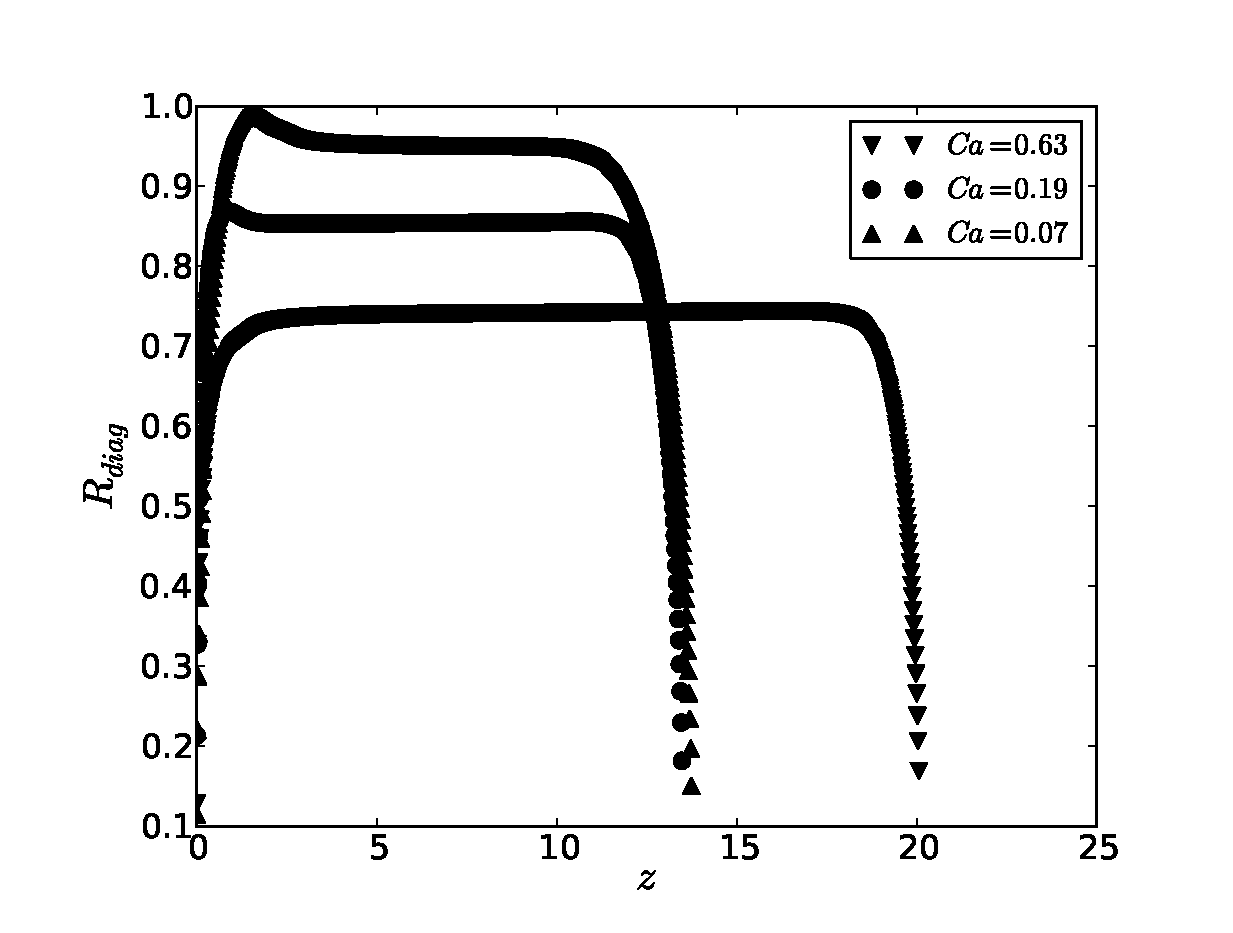
\includegraphics[width=0.8\textwidth]{Figures/bubble_rad_diag.eps}\\
\caption{Radii variations along the bubble for different capillary numbers in the plane $x=0$.
One can see that the diagonal radius shows the jump near the bubble rear cap. This agrees with the
VOF simulations of \citet{wang-non-circular}.Coordinate $z$ increases in the streamwise direction.
\label{fig:bubble:variation:capillaries}}
\end{figure}

Another interesting phenomenon regarding the bubble shape was indicated by \citet{heil-threedim}. In
their simulations the non-axisymmetric shape was observed even for larger capillary numbers $Ca>4$
near
the bubble front cap which after certain distance relaxes to have radii equal to each other. The
bubble shape was calculated for the large capillary number $Ca=6.43$, see Fig.
\ref{fig:bubble:ca:large}. However, even the diagonal radius shows the jump near the front tip of
the bubble and it resembles the shape given by \citet{heil-threedim}, but the difference is around
$1$ percent and can be explained by error in the linear interpolation used for the
interface
calculation. Therefore, we do not observe the symmetry breakage for $Ca>4$. 
\begin{figure}[ht]
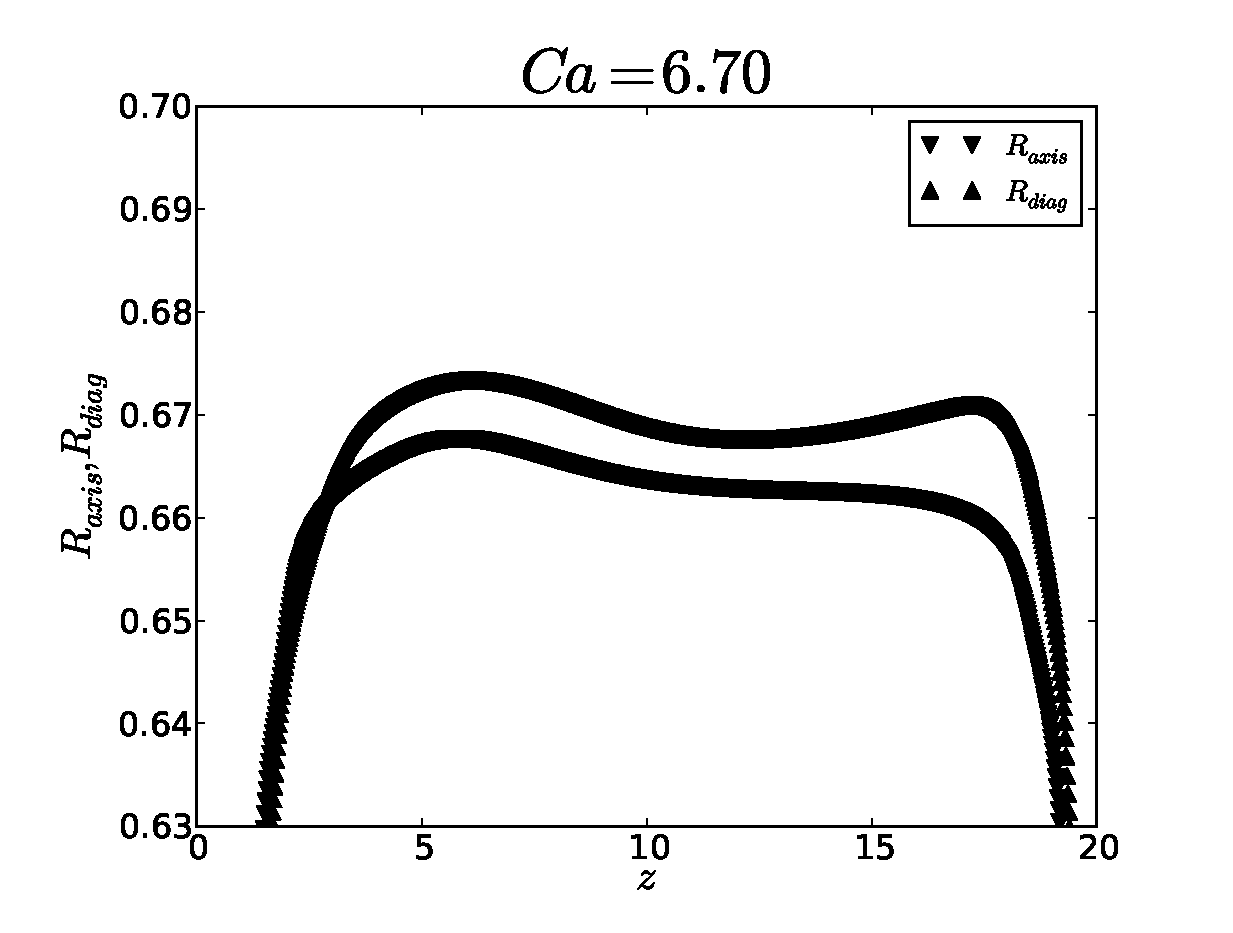
\includegraphics[width=\textwidth]{Figures/bubble_ca_large.eps}
\caption{The bubble shape for the capillary number $Ca=6.43$ is presented. $z$ increases in the
streamwise direction. One can see that near the front tip (large $z$) the diagonal radius exhibits
a jump which is relaxed after to the axis radius. Even this resembles
the shape of the curves obtained by \citet{heil-threedim}, but the
difference between radii is around $1$ percent and can be attributed to
the linear interpolation used in the calculation of the interface.\label{fig:bubble:ca:large}}
\end{figure}

\subsection{Capillary number}
The purpose of this section is to study dependence of the radii on the capillary number. The film
thicknesses were extracted from the middle of the bubble. The data presented in Fig.
\ref{fig:capillary:comparison} is simulated with different techniques including different
initialization, and different grids: $52 \times 52 \times 1500$, $82 \times 82 \times 1500$ and $82
\times 82 \time 2400$. All our results are consistent. Therefore one can conclude that for the
capillary number $Ca\geq
0.05$ grid independence is achieved. The results are compared with the results of
\citet{heil-threedim} and of \citet{wang-non-circular}. The data were extracted from the
corresponding references with the help of the program ``Engauge Digitizer''. We observe that
lattice Boltzmann simulations exhibit 
the transition between non-axisymmetric and axisymmetric shape of the bubble. 

The present simulations show that the corresponding critical capillary number is close to
$\widehat{Ca}=0.1$ that agrees with the work of \citet{wang-non-circular} and is different from the
results of \citet{heil-threedim}, $\widehat{Ca}=0.04$. However, in the range of the moderate
capillary numbers our results are closer to the results of \citet{heil-threedim} and exhibit
less noisy trend in radii values and a more accurate transition between non-axisymmetric ans
axisymmetric cases than results of \citet{wang-non-circular}. 
%For moderate capillary numbers $Ca\geq 0.2$, the radii are smaller than the literature results.
%This
%may be caused by the bubble train simulation or the influence of the binary-liquid model. 
\begin{figure}[ht]
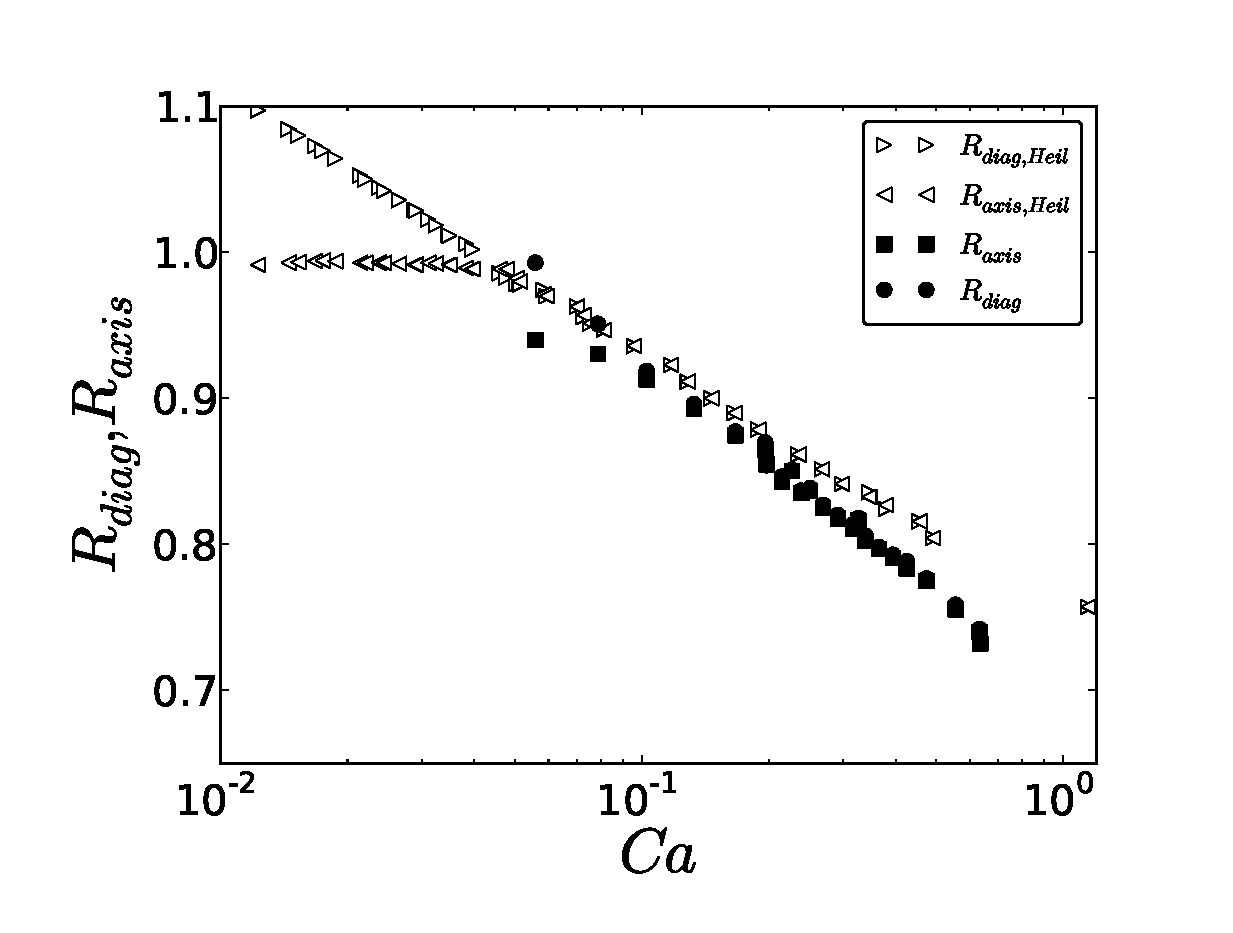
\includegraphics[width=0.8\textwidth]{Figures/capillaries_comparison_heil.eps}\\
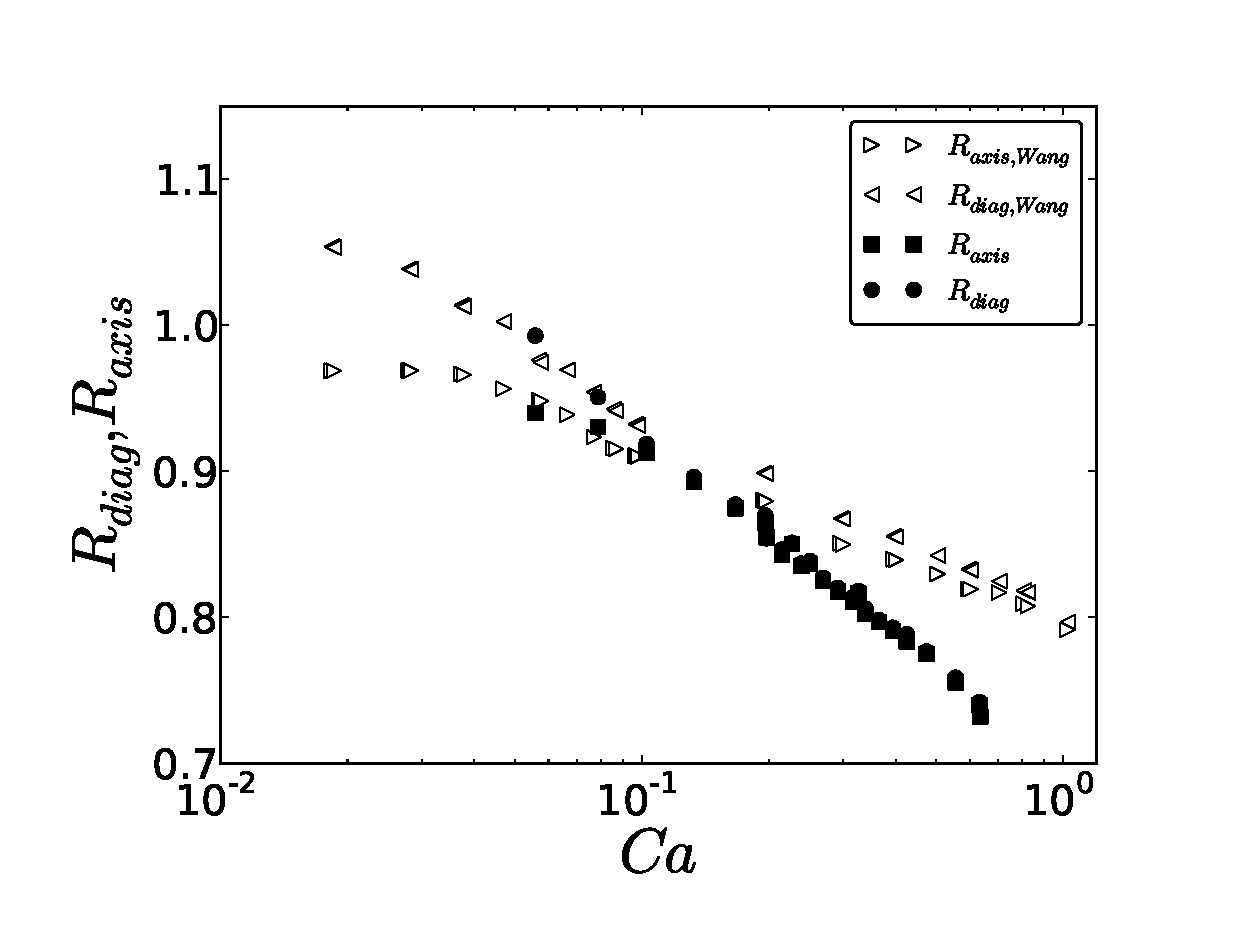
\includegraphics[width=0.8\textwidth]{Figures/capillaries_comparison_wang.eps}\\
\caption{The comparison for the axial and the diagonal radii
versus capillary numbers between present simulations and the results of \citet{heil-threedim}
(top), of \citet{wang-non-circular} (bottom). One can see that
the code mimics
behavior of the earlier published results.  \label{fig:capillary:comparison}} 
\end{figure}

\subsection{Relative velocity}
One of the differencies between the flow in tubes and square capillaries is that the flow has
different streamline patterns. In square microchannels, the main mass flow occurs through corners
\cite{heil-threedim,wang-non-circular}. This affects the mass flow significantly. One of the
characteristics of the mass flow is the normalized dependence of the relative velocity on the
capillary
number. The bubble always moves faster than the surrounding liquid. The following quantity is
defined as
relative velocity \cite{cerro-bubble-train}:
\begin{equation}
W=\frac{U_{\mathrm{bubble}}-U_{ls}}{U_{\mathrm{bubble}}},
\end{equation}
where $U_{\mathrm{bubble}}$ is the bubble interface velocity, and $U_{ls}$ is the liquid superficial
velocity. As far as the steady state is achieved one can take the liquid superficial velocity
exactly at the cross section in the middle between bubbles. The liquid superficial velocity is
defined as:
\begin{equation}
U_{ls}=\frac{\int_{A}{U_{liq}dA}}{A}.
\end{equation}
The relative velocity was calculated and compared with the results of \citet{wang-non-circular},
see Fig. \ref{fig:relative:velocity}. One can see an agreement between the simulations indicating
that
one of the mass transport characteristics can be captured accurately. 
\begin{figure}[ht]
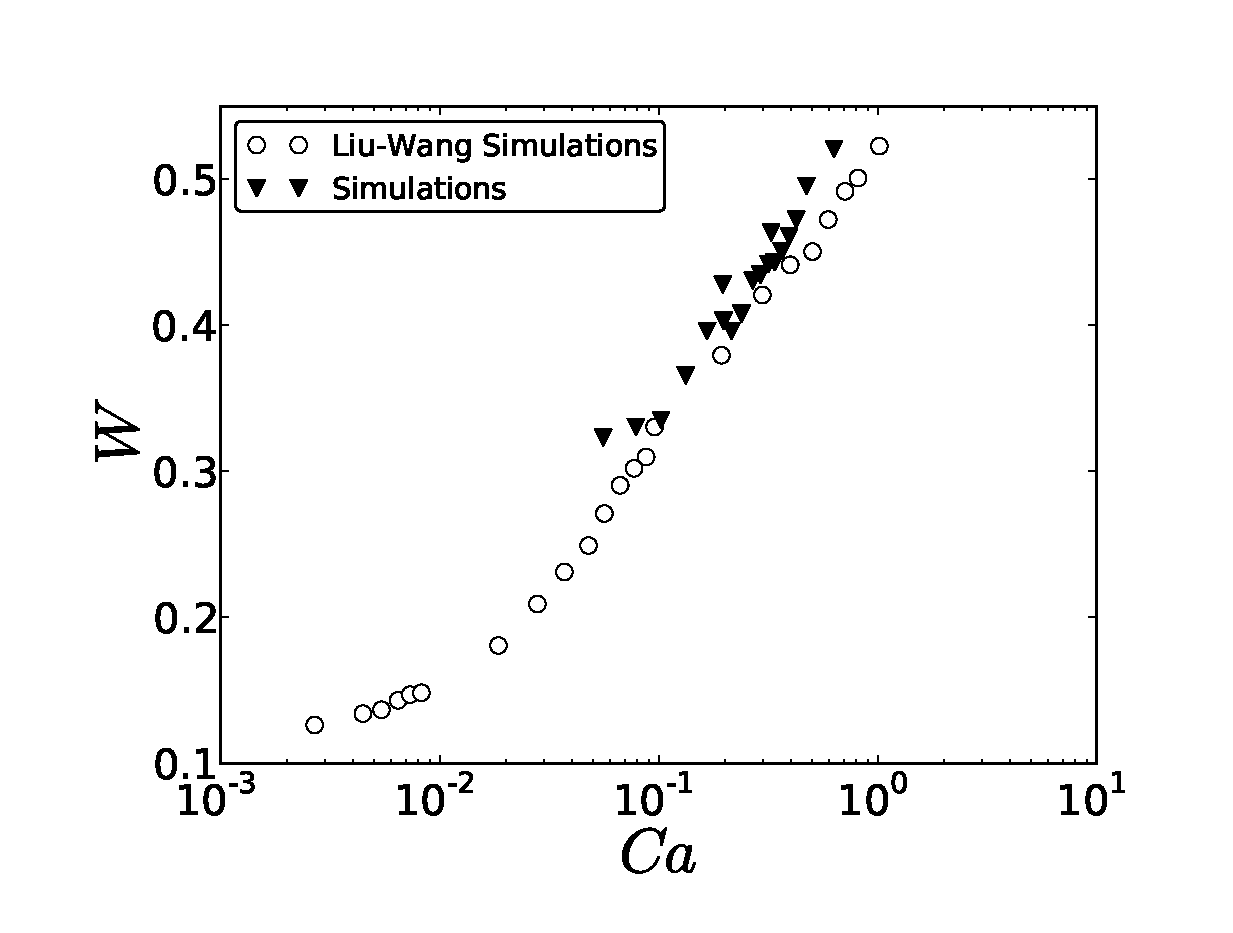
\includegraphics[width=\textwidth]{Figures/relative_velocity.eps}
\caption{Relative velocity comparison between current simulations and simulations of
\citet{wang-non-circular}. One can see a qualitative agreement. \label{fig:relative:velocity}}
\end{figure}

The relative velocity is an important quantity of mass flow characterization
\cite{kreutzer-taylor,yue-mass}. However, there are other important characteristics that
significantly influence the mass transfer, i.e. the frequency of the bubbles \cite{kreutzer-taylor}
and 
inertia effects \cite{heil-bretherton}. 
Future work is planned to study this phenomenon and calculate the mass transfer coefficient by
solving the advection-diffusion equation.
% Preliminary
%studies of the relative velocity show that the binary liquid model can simulate accurately some
%characteristics of mass transfer.

% \section{Train simulation}
% \label{section:bubble:train}
% As far as the requirements for the grid are ``heavy'' we performed a bunch of simulations to
% examine how the distance between bubbles influences on the thickness. For this purpose the
% simulation was conducted on the grid 82x82x750. We examined different initialized distances
%between
% bubbles. The initial lengths of bubbles were chosen as $300$, $350$, $400$, $450$, $500$, $550$
% lattice units. Therefore, the corresponding initial distances between bubbles are
% $450$,$400$,$350$,$300$,$250$ lattice units. On the steady state regime the distances become
%$386$,
% $317$, $248$,$176$,$99$,$23$ lattice units. The corresponding capillary numbers calculated based
%on
% the center bubble velocity are as follows $0.905$, $0.986$,$1.08$,$1.19$, $1.33$, $1.49$. The
% calculated radiuses (diagonal radius equal to the axes radius) are as follows
% $0.783$,$0.778$,$0.772$,$0.764$,$0.753$,$0.747$. Thus, one can see the great impact of the bubbles
% on each other velocity for the given body force. However, in terms of the film thicknesses those
% numbers look adequate. One can see the film thicknesses dependency on the capillary number for
% simulations obtained by \citet{heil-threedim} and bubble train simulations data in Fig.
% \ref{fig:capillaries:train} and in Fig. \ref{fig:capillary:comparison}. One can see that the
% results are consistent and in a good agreement.
% Therefore, though the bubble train mutual motion influences on the film thickness by increasing
%the
% associated capillary number,  however, the film thickness is in accordance with the capillary
% number correlation. Thus, the decrease of the numerical domain is quantified and can be used to
% obtain the data. However, one should be cautious about the initialization, because the Poiseuille
% flow initialization is deviated even further due to mutual motion of bubbles.
% \begin{figure}
% 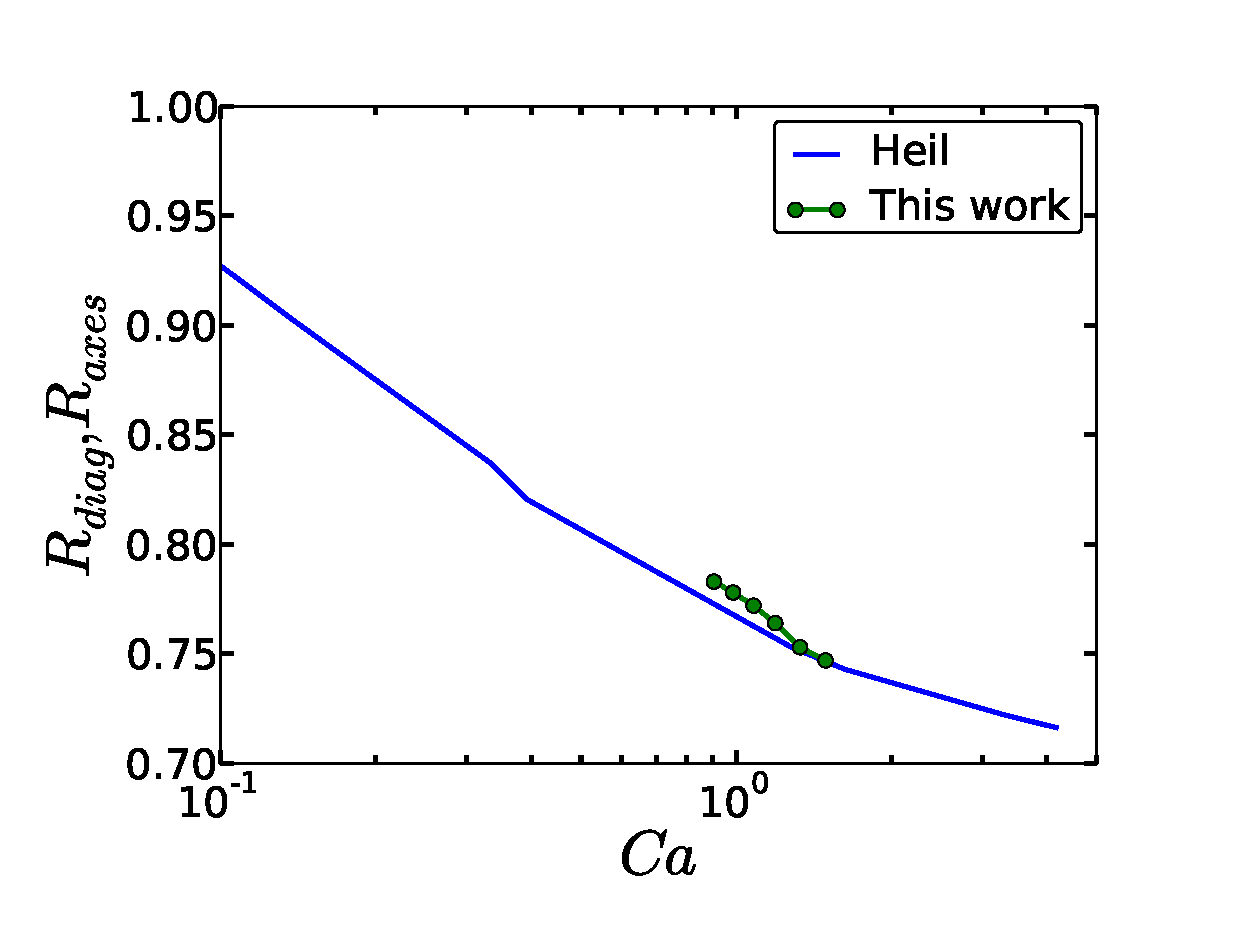
\includegraphics[width=0.97\textwidth]{Figures/capillaries_comparison_train.eps}
% \caption{The comparison for the film thickness between \citet{heil-threedim} data and bubble train
% simulations. Though, one can see that the decrease of the distance between bubbles causes the
% increase in the associated capillary number, however, the correlation dependance between film
% thickness and capillary number stays the same. This can help for simulations to reduce the
% numerical domain. \label{fig:capillaries:train}}
% \end{figure}

\subsection{Rectangular channel simulations}
While the main focus of this paper is on the square microchannel simulations, we performed a number
of simulations for rectangular channels with varying aspect ratio
$\alpha=\frac{W}{H_{\mathrm{eff}}}=\frac{a_x}{a_y}$, where $a_x$ and $a_y$ are sides of the rectangular in $x$ and $y$ directions.\citet{heil-threedim} performed a number of simulations for the
propagation of semi-infinite air finger in the microchannel. They indicated that the radii in $x$
and $y$ directions  are increasing with the aspect ratio $\alpha$
increases. The same trend can be seen for the current simulation results, see Fig.
\ref{fig:aspect:ratio}. One can see that diagonal and axial radii are not the same as they were in square channels for the capillary number range investigated here. The same is
indicated by \citet{heil-threedim} who mentioned that for radii to coincide one needs to have really long bubbles, at least $100$ shorter semi-axis bubble length for the aspect ratio $\alpha=1.5$. This is not possible to achieve with the
current bubble train simulations.
\begin{figure}[htb!]
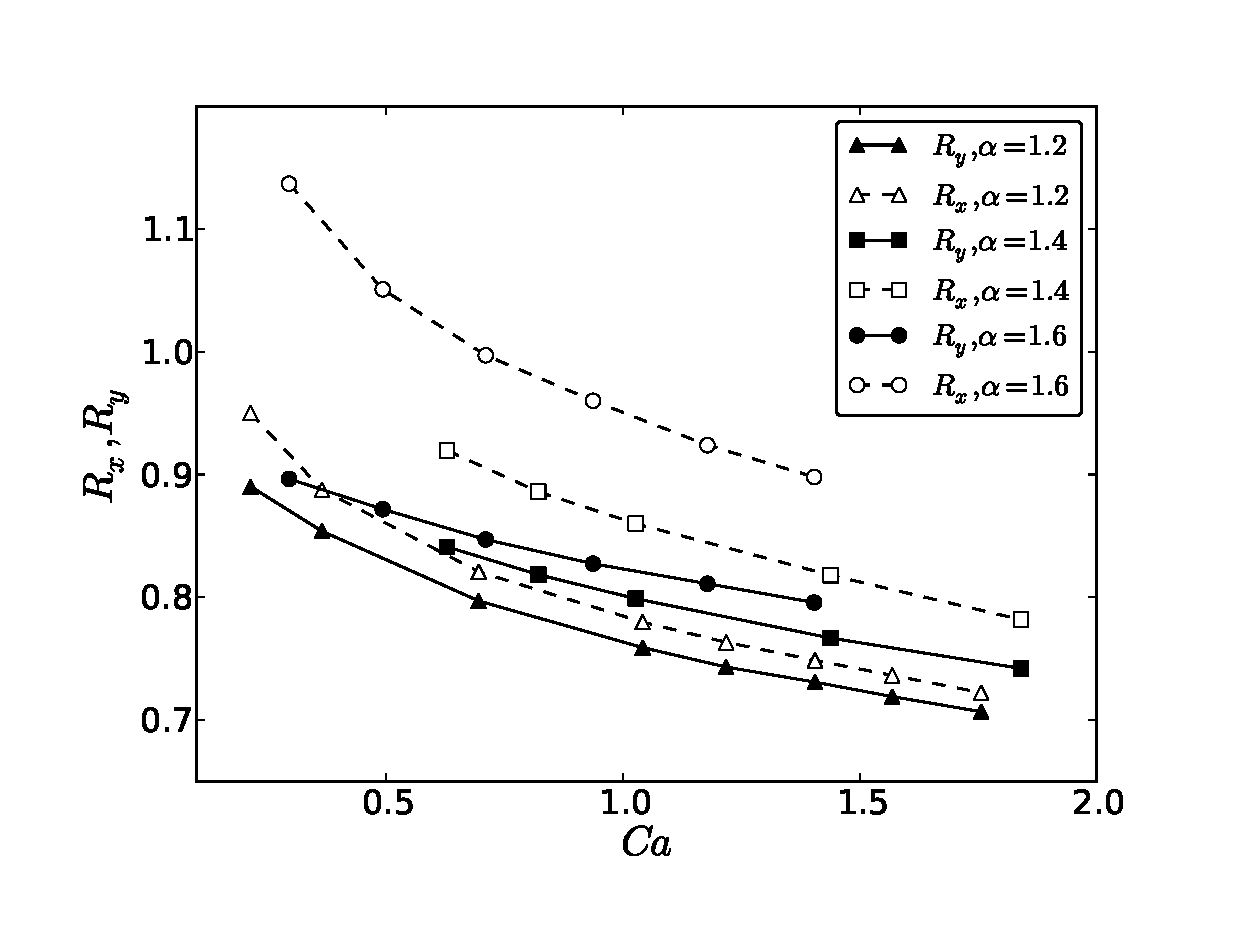
\includegraphics[width=\textwidth]{Figures/rectangle.eps}
\caption{Radii in $x$ ($R_x$) and $y$ ($R_y$) directions for rectangular microchannels with
different aspect ratios. Radii are rescaled on the length of channel in $y$ direction. One can see that with
the increase of $\alpha$ the radii increase as well. However, $R_x\neq R_y$. It was indicated by \citet{heil-threedim} one needs semi-infinite bubble to achieve $R_x=R_y$. \label{fig:aspect:ratio}}
\end{figure}

They as well indicated that the simulations results with different aspect ratio can be
put on one curve by calculating non-dimensional radius $s_{\infty}$ that scales different aspect
ratio microchannels. It is based on the calculation of  $r_{\infty}$ (the radius that the air
finger will have at an infinite distance from the bubble tip):
\begin{equation}
\begin{aligned}
&\frac{r_{\infty}}{\frac{H_{\mathrm{eff}}}{2}}=\frac{\sqrt{\frac{Q}{\pi}}}{\frac{H_{\mathrm{eff}}}{2
} }\\
&s_{\infty}=\frac{r_{\infty}}{\frac{H_{\mathrm{eff}}}{2}}\alpha^{-1/2},
\end{aligned}
\end{equation}
where $Q$ is the area occupied by air in the crossection. \citet{heil-threedim} indicated a simple
physical interpretation of this phenomena:  providing that air is injected with the same
velocity to the channels with different aspect ratio but the same area, the resulting occupied area by the bubble
should not depend on the aspect ratio. That is quite interesting phenomena indicating that if bubbles are infinite long then they would have the same radius and will be circular. The current results, see Fig. \ref{fig:one:curve} show that
this hypothesis can be extended for bubble train flows with different radii $R_h \neq R_v$. 
\begin{figure}[htb!]
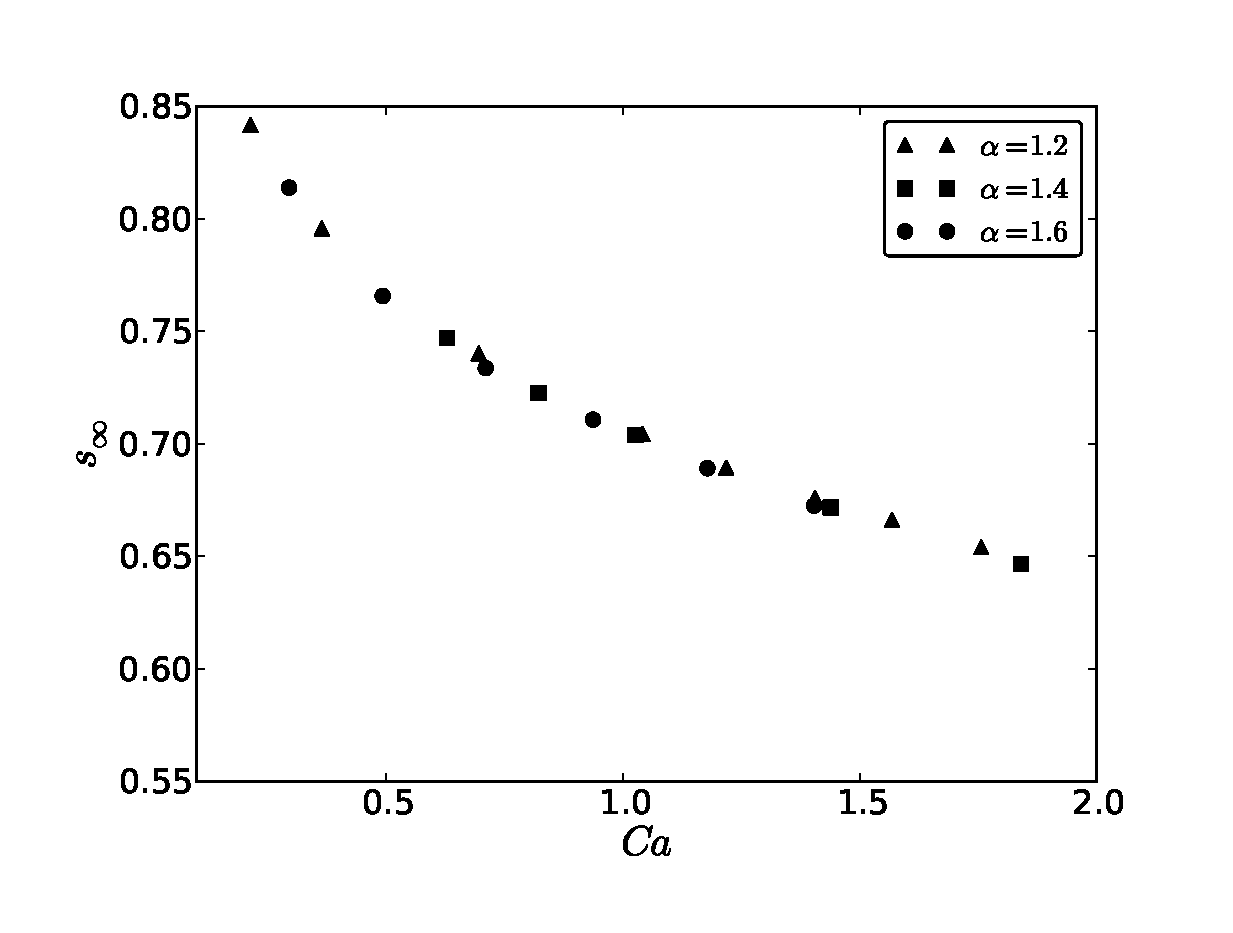
\includegraphics[width=\textwidth]{Figures/onecurve.eps}\\
\caption{The non-dimensional radius $s_{\infty}$ for different aspect ratio
rectangular microchannels. One can see that all the curves coincide
independently of the aspect ratio.\label{fig:one:curve}}
\end{figure}


\section{Conclusion}
This work presents results of binary-liquid simulations for three-dimensional channels with square
cross sections with the lattice Boltzman method. By resolving properly the film thickness as twice the
interface thickness \cite{kuzmin-binary2d} the results were shown to be consistent with those
available in the literature. Note that the literature results show some variations. This work falls
within the range of data presented in the literature. For instance, the  transition from the
non-axisymmetric to the
axisymmetric case is shown to be at $\widehat{Ca}=0.09$ which is close to results of
\citet{wang-non-circular}. However, in the moderate range of parameters simulation results are
close to the results of \citet{heil-threedim} and exhibit more accurate transition between
non-axisymmetric and symmetric cases than results of \citet{wang-non-circular}. Overall, the film
thickness dependency on the capillary number, the
transition from the non-axisymmetric to symmetric case, and the velocity patterns were investigated.
While
the goal of this work is a feasibility study, more numerical studies are needed to
understand the influence of the slug length, inertia effects, pressure distributions
\cite{kreutzer-taylor,yue-mass} on the design of microchannels. Our results show that the lattice
Boltzmann binary liquid model can be used for simulation of gas bubbles in microchannels. 
%Results
%coincide with bulk literature results. 

\appendix
\section{Scaling procedure}
\label{append:scaling}
The scaling procedure has been extensively  described in our previous work \cite{kuzmin-binary2d}.
Here, we present
only an outline of how the simulations are initialized:
\begin{description}
 \item[Capillary number] One first needs to set the capillary number and the Reynolds number for
simulations. 
 \item[Film thickness] After the capillary number is prescribed, one needs to approximate the axial
bubble radius $R_{axial}$, the corresponding film thickness is $\delta=1-R_{axial}$. One can use
correlations of \citet{shikazono-square} or of \citet{kreutzer-taylor}. It can also be done by
taking correlations from numerical simulations by
\citet{heil-bretherton} and \citet{giavedoni-numerical}.  
\item[Grid choice] After specifying the film thickness, one needs to choose the
number of nodes to resolve the film thickness. For binary liquid parameters used in simulations,
$A=0.004,0.04$ and $k=0.004,0.04$ the
interface is spread over approximately $5$ lattice units. To obtain grid independent results one
needs to choose the
film thickness to be $2-2.5$ times larger than the interface thickness \cite{kuzmin-binary2d}.
Given the number of nodes to resolve the film thickness and given the lattice Boltzmann
benchmark, see Section \ref{sec:numerical:benchmark}, one can obtain the grid dimensions.

\item[Velocity] The Reynolds and capillary numbers are supplied from the physical world:
\begin{equation}
\label{definitions:numbers}
\begin{aligned}
&Ca=\frac{U_{\mathrm{bubble}} \mu_{\mathrm{liq}}}{\gamma} \\
&Re=\frac{U_{\mathrm{bubble}} H_{\mathrm{eff}}}{\mu_{\mathrm{liq}}}.
\end{aligned}
\end{equation}
In Eq. \eqref{definitions:numbers} the interface tension coefficient is prescribed by parameters of
the binary liquid model $k$ and $A$, the effective channel height $H_{\mathrm{eff}}$ is obtained
from the film thickness resolution, $\mu_{\mathrm{liq}}$ is defined through the relaxation rate
$\tau_{\mathrm{liq}}$. The relaxation rate $\tau_{liq}$ is prescribed from the gas-liquid viscosity
ratio $\frac{\mu_{\mathrm{liq}}}{\mu_{\mathrm{gas}}}$, where $\mu_{\mathrm{gas}}$ is defined through
the gas relaxation rate $\tau_{\mathrm{gas}}$. The parameter $\tau_{\mathrm{gas}}\geq 0.5$, therefore
 constraining the linked parameter $\tau_{\mathrm{liq}}$. Moreover,
the stability of the lattice Boltzmann scheme is known to deteriorate with the relaxation parameter
$\tau_{\mathrm{liq},\mathrm{gas}}\approx 0.5$ \cite{kuzmin-trt-stability}. On the other hand the
accuracy of the lattice Boltzmann liquid model detiorates as
$\Bigl(\tau_{\mathrm{liq},\mathrm{gas}}-\frac{1}{2}\Bigr)^2$ \cite{ginzburg-trt-simple-hydro}. Thus,
there is a compromise of the choice of parameters $\tau_{\mathrm{liq}}$ and $\tau_{\mathrm{gas}}$.
The gas-liquid viscosity ratio in the current simulations was chosen as
$\frac{\mu_{\mathrm{liq}}}{\mu_{\mathrm{gas}}}=\frac{\nu_{\mathrm{liq}}}{\nu_{\mathrm{gas}}}=10$ and
the relaxation parameters were chosen to be
in the safe region, i.e. $\tau_{liq}=2.5$ and $\tau_{gas}=0.7$. 

Given the considerations of the relaxation parameters, one can obtain the desired bubble velocity
$U_{\mathrm{bubble}}$ from the equation for the Reynolds number (\ref{definitions:numbers}).
Substituting the bubble velocity $U_{\mathrm{bubble}}$ to the definition of the capillary number,
Eq. (\ref{definitions:numbers}), one can obtain the interface tension which is connected with the
binary liquid parameters $k$ and $A$. The stability of the lattice Boltzmann scheme implies the
simultaneous change of $\tau_{\phi}$ with the change of parameters $k$ and $A$
\cite{pagonabarraga-parameters}. Therefore, if Reynolds number is less than
$50-100$ one can neglect the inertia effects and obtain the bubble velocity straight from the
capillary number limiting the complex interplay of the parameters for the LBM simulations to be
stable: 
\begin{equation}
\begin{aligned}
&U_{\mathrm{bubble}}=Ca \frac{\gamma}{\mu_{\mathrm{liq}}}=Ca \frac{\sqrt{\frac{8 k
A}{9}}}{\frac{1}{3}(\tau_{\mathrm{liq}}-\frac{1}{2})}\\
\end{aligned}
\end{equation}
where usually $k=A=0.004,0.04$.

\item[Body force] 
It is desired to obtain the prescribed velocity $U_{\mathrm{bubble}}$ in simulations. Since the
flow in the simulations is driven by a body force, a connection between this force and the
bubble velocity $U_{\mathrm{bubble}}$ has to be established. We assume that the
flow is close to the planar Poiseuille flow with $U_{\mathrm{bubble}}$ being the maximum in the
Poiseuille profile for the square shaped microchannels:
\begin{equation}
\label{poiseuille:square:profile}
\dfrac{\mathrm{d}P}{\mathrm{d}z}=\frac{\mu_{\mathrm{liq}} U_{\mathrm{bubble}}}{\sum_{i\leq 0,j\leq
0}{\dfrac{16}{\pi^6} \dfrac{(-1)^i (-1)^j}{(2 i+1)(2 j+1)\bigl[\frac{(2 i
+1)^2}{W_{\mathrm{eff}}^2}+\frac{(2 j+1)^2}{H_{\mathrm{eff}}^2}\bigr]}}}.
\end{equation}
Though the Poiseuille profile assumption works reasonably well \cite{kuzmin-binary2d}, instead of
calculating sums (\ref{poiseuille:square:profile}) we suggest to simply start simulations with the
body force $\frac{\mathrm{d}P}{\mathrm{d}z}=10^{-6}-10^{-5}$ for grids of size $50\times 50 \times
1500$ and the capillary number $Ca\approx0.1-6.0$.  
\end{description}
After imposing the body force the simulations can be run. A typical simulation runs approximately
$100000-300000$ time steps to reach steady-state, see Section \ref{sec:steady:state}. To design the
simulations one needs to keep proportionality between parameters through the equations above. For
example if one knows the capillary number $Ca_1$ and the corresponding body force
$\frac{\mathrm{d}P_1}{\mathrm{d}z}$ for simulations conducted on the grid with the characteristic
number of nodes $N_{y1}$ , the body force for another simulation can be calculated as:
\begin{equation}
\dfrac{\dfrac{\mathrm{d}P_1}{\mathrm{d}x}}{\dfrac{\mathrm{d}P_2}{\mathrm{d}x}}=\frac{Ca_1}{Ca_2}
\frac{N_{
y2}^2 }{N_{y1}^2}
\end{equation}

\section{Symmetric boundary conditions}
\label{append:sym}
To reduce the computational load in terms of memory and CPU power by a factor of 4, we performed the simulation of 
only a quarter of the channel using symmetric boundary conditions.  The scalar macroscopic variables
at the boundary nodes have the same values as those of the adjacent fluid nodes.  The same applies
for tangential velocities $U_{\tau}$, while velocities perpendicular  to the mirror boundary $U_n$ have opposite signs
to that of the velocity of the fluid node.  This can be summarised as:
\begin{equation}
\rho_B = \rho_F, \quad \phi_B = \phi_F \quad U_{B\tau}=U_{F\tau}, U_{B n}=U_{F n}, 
\end{equation}
where the subscripts $B$ and $F$ stand for the boundary and the nearest fluid node, respectively.

For the lattice Boltzmann model the incoming populations on the boundary node need to be specified.
For generality we assume that the symmetry plane is $\alpha=0$, where $\alpha$ is the
direction $x$ or $y$. Then, for lattice Boltzmann populations the symmetric boundary conditions can
be expressed through the following steps:
\begin{description}
\item[I] Identify complementary directions. For the direction $i'$ to be complementary to the $i$-th
direction, the following relations must hold:
\begin{equation}
\begin{aligned}
&c_{i\alpha}=-c_{i'\alpha}, \text{ where $\alpha=$ is the symmetry plane }\\
&c_{i\beta}=-c_{i'\beta}, \text{ where $\beta\neq\alpha$ }
\end{aligned}
\end{equation}

Note that the complementary directions for the directions parallel to the symmetry plane coincide
with the original direction.

\item[II] Take the distributions from the nearest fluid node and
apply them to the boundary node utilizing the complementary directions:
\begin{equation}
f_{i,B}=f_{i',F}.
\end{equation}
\end{description}

It can easily be seen that the procedure described above conserves the scalar fields and the tangential
velocity, while reversing the normal flux. The plane of symmetry is located half-way between fluid
and boundary nodes. 
\bibliographystyle{unsrtnat}
\bibliography{paper}
\end{document}


